\documentclass[11pt,]{article}
\usepackage{lmodern}
\usepackage{amssymb,amsmath}
\usepackage{ifxetex,ifluatex}
\usepackage{fixltx2e} % provides \textsubscript
\ifnum 0\ifxetex 1\fi\ifluatex 1\fi=0 % if pdftex
  \usepackage[T1]{fontenc}
  \usepackage[utf8]{inputenc}
\else % if luatex or xelatex
  \ifxetex
    \usepackage{mathspec}
  \else
    \usepackage{fontspec}
  \fi
  \defaultfontfeatures{Ligatures=TeX,Scale=MatchLowercase}
    \setmainfont[]{Arial}
    \setsansfont[]{Arial}
    \setmonofont[Mapping=tex-ansi]{Courier}
\fi
% use upquote if available, for straight quotes in verbatim environments
\IfFileExists{upquote.sty}{\usepackage{upquote}}{}
% use microtype if available
\IfFileExists{microtype.sty}{%
\usepackage{microtype}
\UseMicrotypeSet[protrusion]{basicmath} % disable protrusion for tt fonts
}{}
\usepackage[margin=1in]{geometry}
\usepackage{hyperref}
\PassOptionsToPackage{usenames,dvipsnames}{color} % color is loaded by hyperref
\hypersetup{unicode=true,
            pdftitle={MAGenTA: Microbial Assessment by Genome-wide Tn-Seq Analysis},
            pdfauthor={Margaret Antonio, Katherine McCoy, Tim van Opijnen, PhD},
            colorlinks=true,
            linkcolor=blue,
            citecolor=Blue,
            urlcolor=blue,
            breaklinks=true}
\urlstyle{same}  % don't use monospace font for urls
\usepackage{color}
\usepackage{fancyvrb}
\newcommand{\VerbBar}{|}
\newcommand{\VERB}{\Verb[commandchars=\\\{\}]}
\DefineVerbatimEnvironment{Highlighting}{Verbatim}{commandchars=\\\{\}}
% Add ',fontsize=\small' for more characters per line
\usepackage{framed}
\definecolor{shadecolor}{RGB}{248,248,248}
\newenvironment{Shaded}{\begin{snugshade}}{\end{snugshade}}
\newcommand{\KeywordTok}[1]{\textcolor[rgb]{0.13,0.29,0.53}{\textbf{{#1}}}}
\newcommand{\DataTypeTok}[1]{\textcolor[rgb]{0.13,0.29,0.53}{{#1}}}
\newcommand{\DecValTok}[1]{\textcolor[rgb]{0.00,0.00,0.81}{{#1}}}
\newcommand{\BaseNTok}[1]{\textcolor[rgb]{0.00,0.00,0.81}{{#1}}}
\newcommand{\FloatTok}[1]{\textcolor[rgb]{0.00,0.00,0.81}{{#1}}}
\newcommand{\ConstantTok}[1]{\textcolor[rgb]{0.00,0.00,0.00}{{#1}}}
\newcommand{\CharTok}[1]{\textcolor[rgb]{0.31,0.60,0.02}{{#1}}}
\newcommand{\SpecialCharTok}[1]{\textcolor[rgb]{0.00,0.00,0.00}{{#1}}}
\newcommand{\StringTok}[1]{\textcolor[rgb]{0.31,0.60,0.02}{{#1}}}
\newcommand{\VerbatimStringTok}[1]{\textcolor[rgb]{0.31,0.60,0.02}{{#1}}}
\newcommand{\SpecialStringTok}[1]{\textcolor[rgb]{0.31,0.60,0.02}{{#1}}}
\newcommand{\ImportTok}[1]{{#1}}
\newcommand{\CommentTok}[1]{\textcolor[rgb]{0.56,0.35,0.01}{\textit{{#1}}}}
\newcommand{\DocumentationTok}[1]{\textcolor[rgb]{0.56,0.35,0.01}{\textbf{\textit{{#1}}}}}
\newcommand{\AnnotationTok}[1]{\textcolor[rgb]{0.56,0.35,0.01}{\textbf{\textit{{#1}}}}}
\newcommand{\CommentVarTok}[1]{\textcolor[rgb]{0.56,0.35,0.01}{\textbf{\textit{{#1}}}}}
\newcommand{\OtherTok}[1]{\textcolor[rgb]{0.56,0.35,0.01}{{#1}}}
\newcommand{\FunctionTok}[1]{\textcolor[rgb]{0.00,0.00,0.00}{{#1}}}
\newcommand{\VariableTok}[1]{\textcolor[rgb]{0.00,0.00,0.00}{{#1}}}
\newcommand{\ControlFlowTok}[1]{\textcolor[rgb]{0.13,0.29,0.53}{\textbf{{#1}}}}
\newcommand{\OperatorTok}[1]{\textcolor[rgb]{0.81,0.36,0.00}{\textbf{{#1}}}}
\newcommand{\BuiltInTok}[1]{{#1}}
\newcommand{\ExtensionTok}[1]{{#1}}
\newcommand{\PreprocessorTok}[1]{\textcolor[rgb]{0.56,0.35,0.01}{\textit{{#1}}}}
\newcommand{\AttributeTok}[1]{\textcolor[rgb]{0.77,0.63,0.00}{{#1}}}
\newcommand{\RegionMarkerTok}[1]{{#1}}
\newcommand{\InformationTok}[1]{\textcolor[rgb]{0.56,0.35,0.01}{\textbf{\textit{{#1}}}}}
\newcommand{\WarningTok}[1]{\textcolor[rgb]{0.56,0.35,0.01}{\textbf{\textit{{#1}}}}}
\newcommand{\AlertTok}[1]{\textcolor[rgb]{0.94,0.16,0.16}{{#1}}}
\newcommand{\ErrorTok}[1]{\textcolor[rgb]{0.64,0.00,0.00}{\textbf{{#1}}}}
\newcommand{\NormalTok}[1]{{#1}}
\usepackage{longtable,booktabs}
\usepackage{graphicx,grffile}
\makeatletter
\def\maxwidth{\ifdim\Gin@nat@width>\linewidth\linewidth\else\Gin@nat@width\fi}
\def\maxheight{\ifdim\Gin@nat@height>\textheight\textheight\else\Gin@nat@height\fi}
\makeatother
% Scale images if necessary, so that they will not overflow the page
% margins by default, and it is still possible to overwrite the defaults
% using explicit options in \includegraphics[width, height, ...]{}
\setkeys{Gin}{width=\maxwidth,height=\maxheight,keepaspectratio}
\IfFileExists{parskip.sty}{%
\usepackage{parskip}
}{% else
\setlength{\parindent}{0pt}
\setlength{\parskip}{6pt plus 2pt minus 1pt}
}
\setlength{\emergencystretch}{3em}  % prevent overfull lines
\providecommand{\tightlist}{%
  \setlength{\itemsep}{0pt}\setlength{\parskip}{0pt}}
\setcounter{secnumdepth}{0}
% Redefines (sub)paragraphs to behave more like sections
\ifx\paragraph\undefined\else
\let\oldparagraph\paragraph
\renewcommand{\paragraph}[1]{\oldparagraph{#1}\mbox{}}
\fi
\ifx\subparagraph\undefined\else
\let\oldsubparagraph\subparagraph
\renewcommand{\subparagraph}[1]{\oldsubparagraph{#1}\mbox{}}
\fi

%%% Use protect on footnotes to avoid problems with footnotes in titles
\let\rmarkdownfootnote\footnote%
\def\footnote{\protect\rmarkdownfootnote}

%%% Change title format to be more compact
\usepackage{titling}

% Create subtitle command for use in maketitle
\newcommand{\subtitle}[1]{
  \posttitle{
    \begin{center}\large#1\end{center}
    }
}

\setlength{\droptitle}{-2em}
  \title{MAGenTA: Microbial Assessment by Genome-wide Tn-Seq Analysis}
  \pretitle{\vspace{\droptitle}\centering\huge}
  \posttitle{\par}
  \author{Margaret Antonio, Katherine McCoy, Tim van Opijnen, PhD}
  \preauthor{\centering\large\emph}
  \postauthor{\par}
  \predate{\centering\large\emph}
  \postdate{\par}
  \date{25 January 2017}

\usepackage{wrapfig}

\begin{document}
\maketitle

{
\hypersetup{linkcolor=black}
\setcounter{tocdepth}{2}
\tableofcontents
}
\newpage

\section{Introduction}\label{introduction}

\subsection{An Overview of Tn-Seq}\label{an-overview-of-tn-seq}

Tn-Seq is a method of determining quantitative fitnesses of bacterial
genes. This manual is not meant to describe it in full, only how to
analyze the sequencing data it produces. For more information on Tn-Seq,
several papers
\href{http://www.nature.com/nmeth/journal/v6/n10/abs/nmeth.1377.html}{1},
\href{http://www.nature.com/nrmicro/journal/v11/n7/abs/nrmicro3033.html}{2},
\href{http://www.ncbi.nlm.nih.gov/pmc/articles/PMC3514683/}{3},
\href{http://journals.plos.org/plospathogens/article?id=10.1371/journal.ppat.1005869}{4})
have been published with detailed explanations. To begin, the tools and
steps used to process the sequence data depend on how the sequences were
prepared (Fig. 1).

\centerline{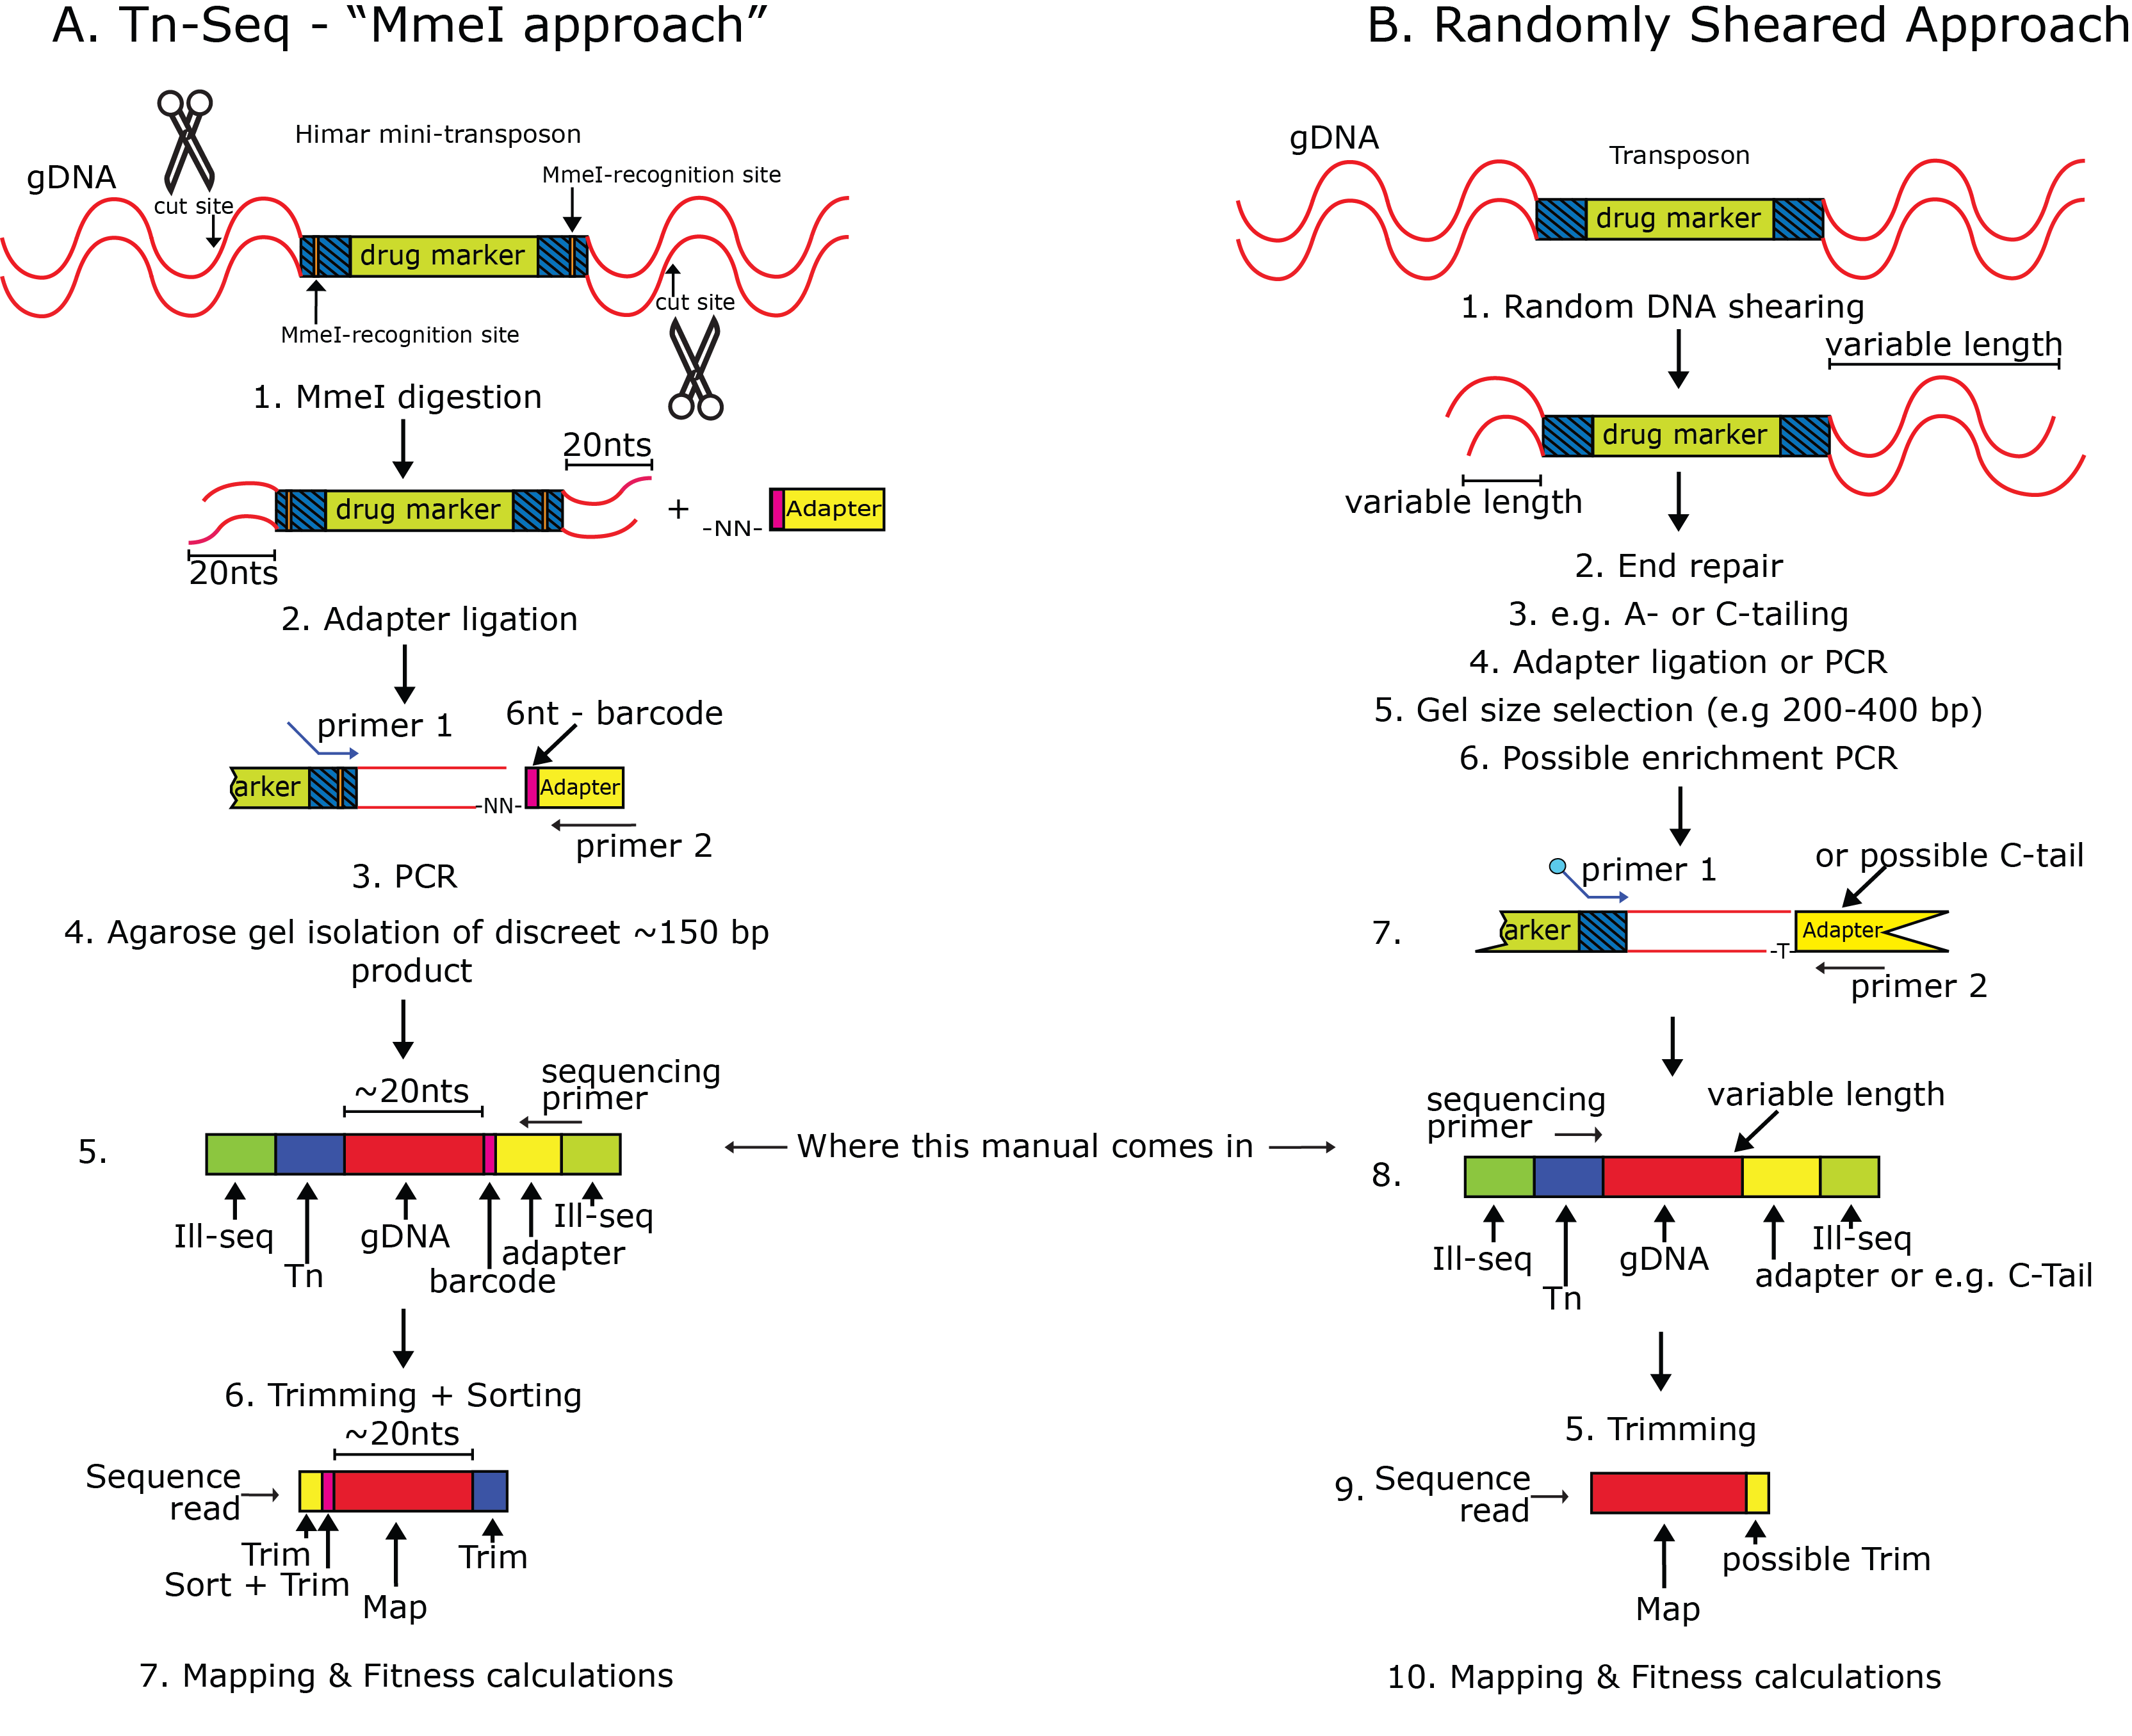
\includegraphics[width=0.8\linewidth]{figs/sequence.png}}

\noindent
\textbf{Figure 1.} \textbf{Two approaches to Tn-Seq sample preparation.}
(A) The
\href{http://www.nature.com/nmeth/journal/v6/n10/abs/nmeth.1377.html}{MmeI
Tn-Seq procedure} uses MmeI digestion to generate a PCR product of
approximately 150bp, with two flanking sequences necessary for Illumina
sequencing (in green), a small piece of the transposon sequence (in
blue), approximately 20nts of bacterial genomic DNA (gDNA; in red), and
the adapter sequence (in yellow), which also contains a six nucleotide
barcode to enable multiplexing (in pink). Note that in this approach
sequencing starts from the sequencing primer on the right then reads
into the barcode, the gDNA, and finally the transposon. (B)
Alternatively, gDNA is randomly sheared so that the product to be
sequenced has a variable length. It is unclear how large the gDNA
fragment is; sequencing starts from the transposon side, reads into the
gDNA, and depending on the size of the gDNA may read into the adapter or
C-tail.

\subsection{Workflow}\label{workflow}

Following sequencing of reads from either approach in Figure 1, the
reads are processed, fitness costs of single mutations are calculated,
and comparative analyses can be performed (Fig. 2).

\centerline{\includegraphics[width=0.8\linewidth]{figs/tnseq.png}}

\noindent
\textbf{Figure 2.} \textbf{An overview of the main steps of Tn-Seq Data
Pre-processing and MAGenTA Anlayses.} In Part A: ``Data Prep'', all
non-genomic parts of the sequences are removed and the remaining
sequence is mapped to the reference genome. In Part B: ``Fitness
Analysis'', the differences in mapped reads between an initial time
point and a second time point are used to calculate the fitness of
single insertions, which can then be aggregated over regions in a
gene-centric or non-genecentric analysis. Finally, Part C: ``Comparative
Analyses \& Other Tools'' includes optional analyses for comparing and
visualizing fitness data. \pagebreak

\section{Part A: Data Prep}\label{part-a-data-prep}

\subsection{Input Files}\label{input-files}

The following inputs are used in Part 1 of Tn-Seq data processing:

\begin{enumerate}
\def\labelenumi{\arabic{enumi}.}
\item
  \textbf{Sequencing reads} in
  \href{http://maq.sourceforge.net/fastq.shtml}{FASTQ format}. These
  files should end in .fastq and look like
  \href{https://en.wikipedia.org/wiki/FASTQ_format}{this}:

\begin{verbatim}
@SRR001666.1 071112_SLXA-EAS1_s_7:5:1:817:345 length=72
GGGTGATGGCCGCTGCCGATGGCGTCAAATCCCACCAAGTTACCCTTAACAACTTAAGGGTTTTCAAATAGA
+SRR001666.1 071112_SLXA-EAS1_s_7:5:1:817:345 length=72
IIIIIIIIIIIIIIIIIIIIIIIIIIIIII9IG9ICIIIIIIIIIIIIIIIIIIIIDIIIIIII>IIIIII/
@SRR001666.2 071112_SLXA-EAS1_s_7:5:1:801:338 length=72
GTTCAGGGATACGACGTTTGTATTTTAAGAATCTGAAGCAGAAGTCGATGATAATACGCGTCGTTTTATCAT
+SRR001666.2 071112_SLXA-EAS1_s_7:5:1:801:338 length=72
IIIIIIIIIIIIIIIIIIIIIIIIIIIIIIII6IBIIIIIIIIIIIIIIIIIIIIIIIGII>IIIII-I)8I
\end{verbatim}
\item
  \textbf{Expansion factors}, experimentally determined integers
  representing expansion of the bacterial populations under study. One
  method of determining the expansion factor is to divide the number of
  bacteria at the end of an experiment by the number at the beginning of
  the experiment. In vitro, assessing bacteria population size is
  conventially performed by counting colony forming units (CFUs) in
  serial dillutions. A method for in vivo determination of expansion
  factor is discussed
  \href{http://www.ncbi.nlm.nih.gov/pmc/articles/PMC3514683/}{here}.
\item
  \textbf{\href{http://hannonlab.cshl.edu/fastx_toolkit/commandline.html\#fastx_barcode_splitter_usage}{Barcodes}},
  listed in a text (.txt) file, formatted as follows: one barcode per
  line with the barcode name and sequence tab-delimited. Barcodes are
  often only used to differentiate between different libraries or
  experimental conditions. This file can be created in any plain text
  editor, with one barcode per line: an arbitrary barcode name, a tab,
  and the barcode sequence. It is recommended that the barcode names be
  descriptive, including library number, expansion factor, and
  experimental condition for better identification. A sample barcode.txt
  file:

\begin{verbatim}
L1_2394e_Glucose  ACTGAC
L2_2394e_Glucose  CTGACT
L3_2394e_Glucose  GACTGA
L1_350e_Penn  GGACGA
L2_350e_Penn TACTTG
L3_350e_Penn  ATGAAC
\end{verbatim}
\item
  \textbf{Additional barcodes for the MmeI approach}. If using the MmeI
  Tn-Seq approach, four additional barcode files which describe the end
  of the MmeI transposon sequence are required. As shown below, there is
  a variable region of adaptor DNA in each read, which is identified in
  the barcode for trimming. As in the previous barcode file, this should
  be in tab-delimited format, ending in .txt, with one barcode per line,
  per file. An example of four such barcode files are shown
  \href{https://github.com/vanOpijnenLab/magenta-p2/tree/master/example\%20files}{here}.
  Each of the barcode files contain one of the following lines:

\begin{verbatim}
trim1 TAA
trim2 TAAC
trim3 TAACA
trim4 TAACAG
\end{verbatim}
\item
  \textbf{\href{https://www.ncbi.nlm.nih.gov/Sitemap/samplerecord.html}{Genbank}
  and \href{http://zhanglab.ccmb.med.umich.edu/FASTA/}{FASTA} files}
  (follow the links for examples of genbank and fasta format files) for
  each strain being analyzed. Both can be found on
  \href{https://www.ncbi.nlm.nih.gov/pubmed}{NCBI} by searching for each
  strain under the Genome section. For example, on the
  \href{https://www.ncbi.nlm.nih.gov/genome/?term=streptococcus+pneumoniae}{genome
  page here} for \emph{Streptococcus Pneumoniae R6} in NCBI, at the top
  box, there are links to download Genbank and Fasta formats of the
  organism's genome. These files should end in .gbk and .fasta
  respectively. Note that even though the Galaxy and Command-line tools
  we describe in this manual can open and read these files, typically if
  one just clicks the file to open it, the computer cannot automatically
  detect which program to use to open fasta and genbank files. To view
  the file before using it, simply change the file extension from
  ``.gbk'' or ``.fasta'' to ``.txt''. This way a regular text editor
  will open it.
\end{enumerate}

\textbf{An example of the first five lines and a few lines from the
first annotated gene of a typical genbank file are shown:}

\begin{verbatim}
LOCUS       NC_012469            2112148 bp    DNA     circular CON 10-JUN-2013
DEFINITION  Streptococcus pneumoniae Taiwan19F-14 chromosome, complete genome.
ACCESSION   NC_012469
VERSION     NC_012469.1  GI:225860012
DBLINK      Project: 59119

...

     source          1..2112148
                     /organism="Streptococcus pneumoniae Taiwan19F-14"
                     /mol_type="genomic DNA"
                     /strain="Taiwan19F-14"
     gene            197..1558
                     /gene="dnaA"
                     /locus_tag="SPT_0001"
                     /db_xref="GeneID:7686582"
     CDS             197..1558
                     /gene="dnaA"
                     /locus_tag="SPT_0001"
                     /note="binds to the dnaA-box as an ATP-bound complex"
                     /codon_start=1
                     /transl_table=11
                     /product="chromosomal replication initiation protein"
                     /protein_id="YP_002741522.1"
                     /db_xref="GI:225860013"
                     /db_xref="GeneID:7686582"
                     /translation="MKEKQFWNRILEFAQERLTRSMYDFYAIQAELIKVEENVATIFL
                     PRSEMEMVWEKQLKDIIVVAGFEIYDAEITPHYIFTKPQDTTSSQVEEATNLTLYDYS
                     PKLVSIPYSDTGLKEKYTFDNFIQGDGNVWAVSAALAVSEDLALTYNPLFIYGGPGLG"
\end{verbatim}

\textbf{An example of the beginning of the beginning of the
Streptoccocus pneumoniae R6 genome in FASTA format is as follows:}

\begin{verbatim}
>NC_003098.1 Streptococcus pneumoniae R6 chromosome, complete genome
TTGAAAGAAAAACAATTTTGGAATCGTATATTAGAATTTGCACAAGAAAGACTGACTCGATCCATGTATGATTTCTATGC
TATTCAAGCTGAACTTATCAAGGTAGAGGAAAATGTTGCCACTATATTTCTACCTCGCTCTGAAATGGAAATGGTCTGGG
AAAAACAACTAAAAGATATTATTGTAGTAGCTGGTTTTGAAATTTATGACGCTGAAATAACTCCCCACTATATTTTCACC
\end{verbatim}

\begin{enumerate}
\def\labelenumi{\arabic{enumi}.}
\setcounter{enumi}{5}
\item
  \textbf{List of normalization genes} for the organism under study.
  Normalization genes are genes that do not affect organismal fitness
  when disrupted. Such genes are generally transposon genes,
  pseudogenes, and degenerate genes. Although a normalization gene file
  is not necessary for running Tn-Seq analysis tools, if the
  normalization genes are known, they should be listed, one per line in
  a text file, ending in .txt. For example, a portion of the
  normalization file for \emph{Streptococcus pneumoniae} TIGR4 is shown
  as follows, with genes listed by their gene id:

\begin{verbatim}
SP_0130
SP_0131
SP_0362
SP_0364
SP_0365
\end{verbatim}
\end{enumerate}

\subsection{Galaxy Toolshed}\label{galaxy-toolshed}

The \href{https://galaxyproject.org/}{Galaxy Project} is a web-based
platform for biomedical research tools. A tutorial on how to set up a
Galaxy environment can be found
\href{https://wiki.galaxyproject.org/Admin/GetGalaxy}{here}, how to
upload files is described
\href{https://wiki.galaxyproject.org/Admin/DataLibraries/UploadingLibraryFiles}{here},
and our custom tools can all be found and installed through the
\href{https://wiki.galaxyproject.org/Admin/Tools/AddToolFromToolShedTutorial}{Galaxy
toolshed}. Currently the custom tools in this pipeline that are
available in the Galaxy Toolshed are:

\begin{itemize}
\tightlist
\item
  enhanced\_bowtie\_mapper
\item
  fastq\_collapser
\item
  calculate\_fitnesses
\item
  aggregate\_fitnesses
\end{itemize}

As described in Figure 1, there are three main parts to the analysis.
Part 1: Data Prep varies depending on the type of input data. If
experimental samples were prepared using the MmeI Tn-Seq method, then
the corresponding data preparation procedure should be followed. An
alternative processing workflow is described for the random shearing
method. In these two cases and if samples were prepared through another
method, the general outline of the workflow is as follows and can be
customized depending on the method used. Create a custom workflow using
Galaxy's
\href{https://wiki.galaxyproject.org/Learn/AdvancedWorkflow}{workflow
editor}:

\begin{enumerate}
\def\labelenumi{\arabic{enumi}.}
\tightlist
\item
  Split data by experimental condition barcodes, if any, using the fastx
  barcode splitter.
\item
  Remove all non-genomic DNA using a tool like the fastq trimmer.
\item
  Filter reads by quality using the fastq quality splitter
\item
  Map reads in Bowtie. We recommend using most standard flags, with the
  following modifications: use best, try hard, discard reads mapping to
  multiple locations, and have the output be in map format (as the
  calc\_fit tool only takes inputs in this format). The number of
  allowed mismatches can be fiddled with, but should be relatively low
  to prevent false mapping.
\end{enumerate}

All output results of Part 1: Data Prep can be used in Part 2 and Part 3
regardless of whether the MmeI or Random Shearing methods were used.

\subsection{MmeI Tn-Seq Prep}\label{mmei-tn-seq-prep}

Download Galaxy Workflows:
\href{https://raw.githubusercontent.com/vanOpijnenLab/magenta-p2/blob/master/workflows/Galaxy-Workflow-MmeI_Tn-Seq_Prep_Pt.1.ga}{Part
1},
\href{https://raw.githubusercontent.com/vanOpijnenLab/magenta-p2/blob/master/workflows/Galaxy-Workflow-MmeI_Tn-Seq_Prep_Pt.2.ga}{Part
2}, and
\href{https://raw.githubusercontent.com/vanOpijnenLab/magenta-p2/blob/master/workflows/Galaxy-Workflow-MmeI_Tn-Seq_Prep_Pt.3.ga}{Part
3}

This prep procedure assumes a 50nt read, as described in Fig. 1 A), with
its first 9 nucleotides from an adaptor, the next six from its barcode,
the next 15 to 18 from genomic DNA, and the last 20 to 23 from its
transposon. In Part 1 it trims the first 9 and last 17, then splits by
the potential segments of transposon DNA (TAA, TAAC, TAACA, or TAACAG)
left on its end using the barcode splitter. In part 2 it trims that
remaining transposon DNA, concatinates the files back into one, and
splits by experimental barcode with the barcode splitter. In Part 3 it
trims the barcodes from the reads and puts the barcode names in the file
names so that they're labeled by experimental condition, filters the
reads, collapses them, and maps them to the genome provided.

\subsubsection{Part 1: Trim \& split by trailing transposon
sequence}\label{part-1-trim-split-by-trailing-transposon-sequence}

\begin{enumerate}
\def\labelenumi{\arabic{enumi}.}
\tightlist
\item
  Navigate to the workflow tab, click on the ``Standard Tn-Seq Prep
  Pt.1'' workflow, and select ``Run''. A workflow should appear with the
  following steps:
\end{enumerate}

\centerline{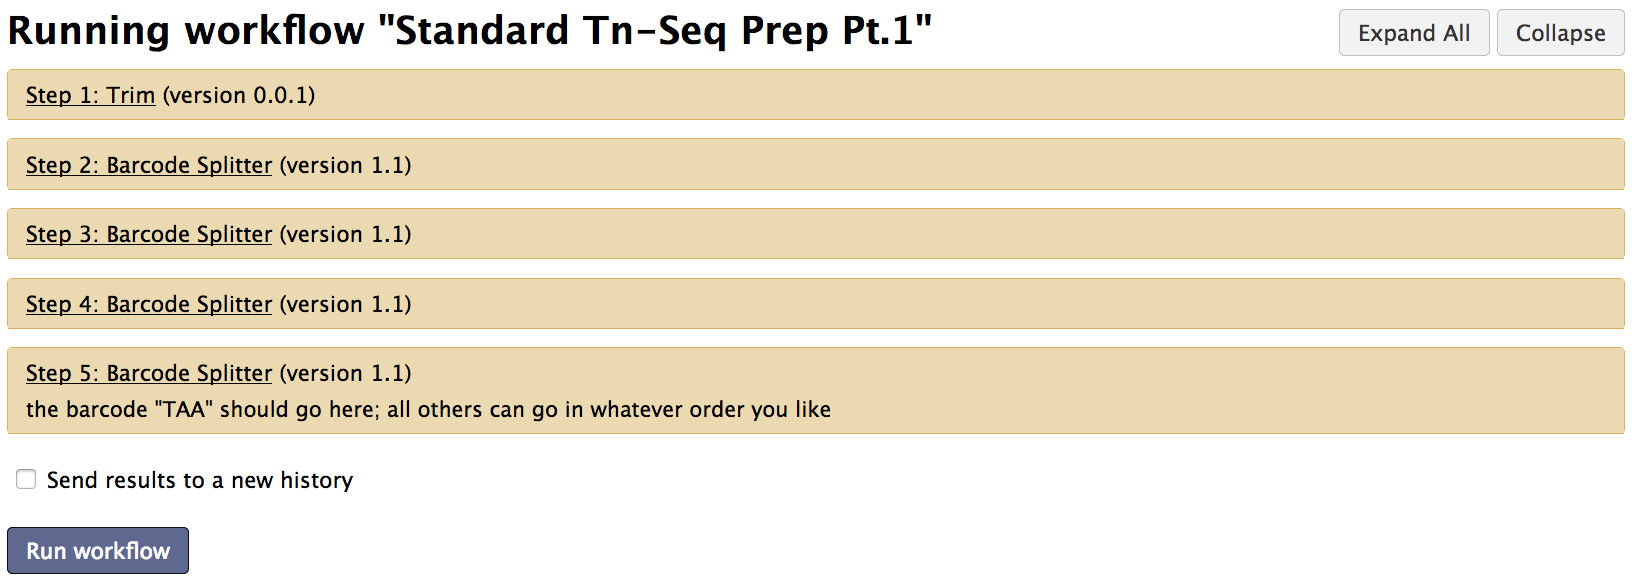
\includegraphics[width=0.8\linewidth]{figs/StandPrep1.png}}

\begin{enumerate}
\def\labelenumi{\arabic{enumi}.}
\setcounter{enumi}{1}
\tightlist
\item
  Select the FASTQ file under ``this dataset'' in ``Step 1: Trim''. The
  default settings will trim of the first 9 and the last 17nts.
\item
  Select the four transposon sequence barcode files in Steps 2 through
  5, one per step. Note that these transposon-endings are entered as
  ``barcodes'' in the workflow, but they are not the experimental
  barcodes, just transposon ends the tool searches for like barcodes.
  They can go in any order, except that the ``trim1'' barcode (finds
  sequences ending in TAA) should go under Step 5, which allows for 0
  mismatches, because it is only 3 bp long so even a single mismatch is
  too loose a constraint.
\item
  Press ``Run workflow'', and wait for the workflow to finish running.
\end{enumerate}

\subsubsection{Part 2: trim trailing transposon sequence, concatenate
files together, and split by
barcode}\label{part-2-trim-trailing-transposon-sequence-concatenate-files-together-and-split-by-barcode}

\begin{enumerate}
\def\labelenumi{\arabic{enumi}.}
\tightlist
\item
  Navigate to the workflow tab, click on the ``Standard Tn-Seq Prep
  Pt.2'' workflow, and select ``Run''. A workflow should appear with the
  following steps:
\end{enumerate}

\centerline{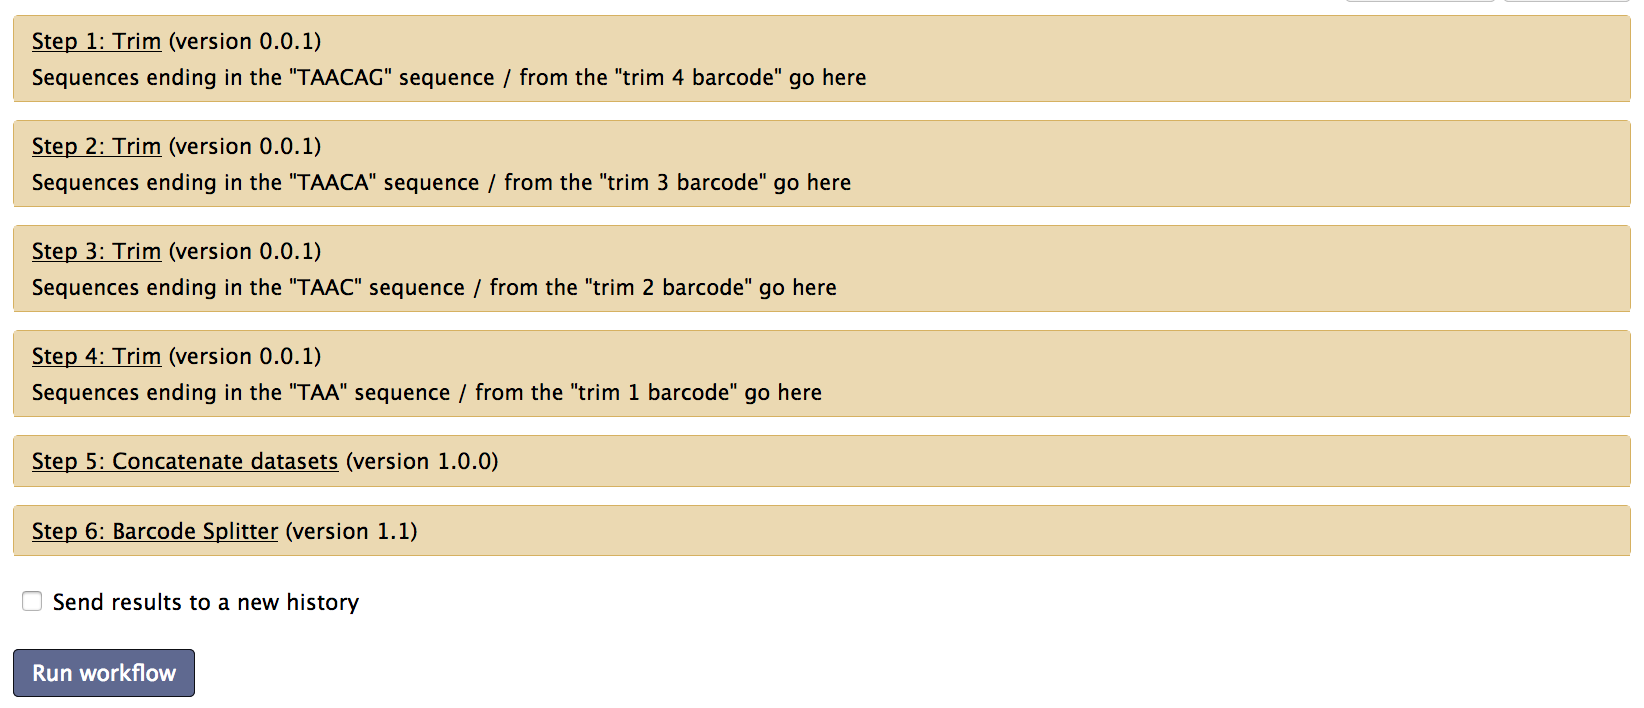
\includegraphics[width=0.8\linewidth]{figs/StandPrep2.png}}

\begin{enumerate}
\def\labelenumi{\arabic{enumi}.}
\setcounter{enumi}{1}
\tightlist
\item
  Select the trim4 barcode-split file under ``this dataset'' for ``Step
  1: Trim'' (the step with ``-4'' under ``Remove everything from this
  position to the end'').
\item
  Select the trim3 barcode-split file under ``this dataset'' for ``Step
  2: Trim'' (the step with ``-3'' under ``Remove everything from this
  position to the end'').
\item
  Select the trim2 barcode-split file under ``this dataset'' for ``Step
  3: Trim'' (the step with ``-1'' under ``Remove everything from this
  position to the end'').
\item
  Select the trim1 barcode-split file under ``this dataset'' for ``Step
  4: Trim'' (the step with ``-2'' under ``Remove everything from this
  position to the end'').
\item
  Select the barcode file under ``Barcodes to use'' in ``Step 6: Barcode
  Splitter''. These should be the barcodes identifying which
  experimental condition each read is from.
\item
  Press ``Run workflow'', and wait for the workflow to finish running.
\item
  Refresh the history and make a list out of the resulting files to send
  into the next workflow, via the ``operations on multiple datasets''
  button located in Galaxy's history sidebar.
\end{enumerate}

\centerline{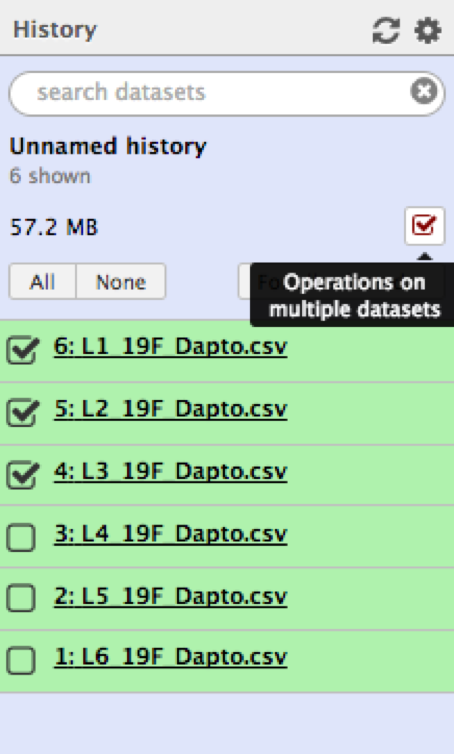
\includegraphics[width=0.25\textwidth]{figs/opButton.png}}

\subsubsection{Part 3: Trim barcode, filter reads by quality, collapse
reads, and map
them}\label{part-3-trim-barcode-filter-reads-by-quality-collapse-reads-and-map-them}

\begin{enumerate}
\def\labelenumi{\arabic{enumi}.}
\tightlist
\item
  Navigate to the workflow tab, click on the ``Standard Tn-Seq Prep
  Pt.3'' workflow, and select ``Run''. A workflow should appear with the
  following steps:
\end{enumerate}

\centerline{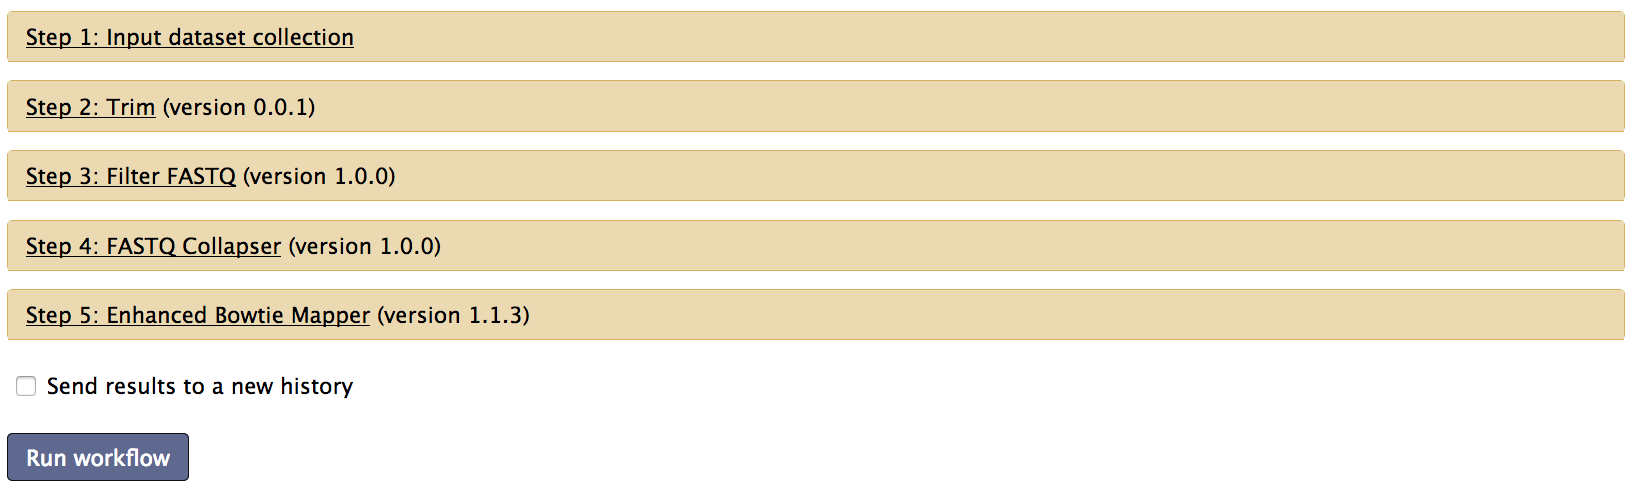
\includegraphics[width=0.8\linewidth]{figs/StandPrep3.png}}

\begin{enumerate}
\def\labelenumi{\arabic{enumi}.}
\setcounter{enumi}{1}
\tightlist
\item
  Under ``Step 5: Map with Bowtie for Illumina'', select the fasta
  genome under ``Select the reference genome''.
\item
  Press ``Run workflow'', and wait for the workflow to finish running.
\end{enumerate}

\subsection{Randomly Sheared Tn-Seq
Prep}\label{randomly-sheared-tn-seq-prep}

\href{https://raw.githubusercontent.com/vanOpijnenLab/magenta-p2/blob/master/workflows/Randomly\%20Sheared\%20Data\%20Prep.ga}{Download
Galaxy Workflow}

As described in Fig. 1 B, another method to prepare a Tn-Seq sample
involves DNA shearing and ligating on C-tails. This prep assumes a 50nt
read of genomic DNA followed by a C-tail, of variable length due to the
randomness of the shearing. It removes the C-tail from the end with
Cutadapt, grooms the reads, filters them for quality, collapses them,
and maps them. If the reads were prepared in this manner but also had
barcodes, the barcode splitter tool should be used to separate them by
barcode first.

\begin{enumerate}
\def\labelenumi{\arabic{enumi}.}
\tightlist
\item
  Use the ``operations on multiple datasets'' button (located in
  Galaxy's history sidebar) to make a list out of all the sequence files
  to be analyzed.
\item
  Navigate to the workflow tab, click on the ``Randomly Sheared Data
  Prep'' workflow, and select ``Run''. A workflow should appear with the
  following steps:
\end{enumerate}

\centerline{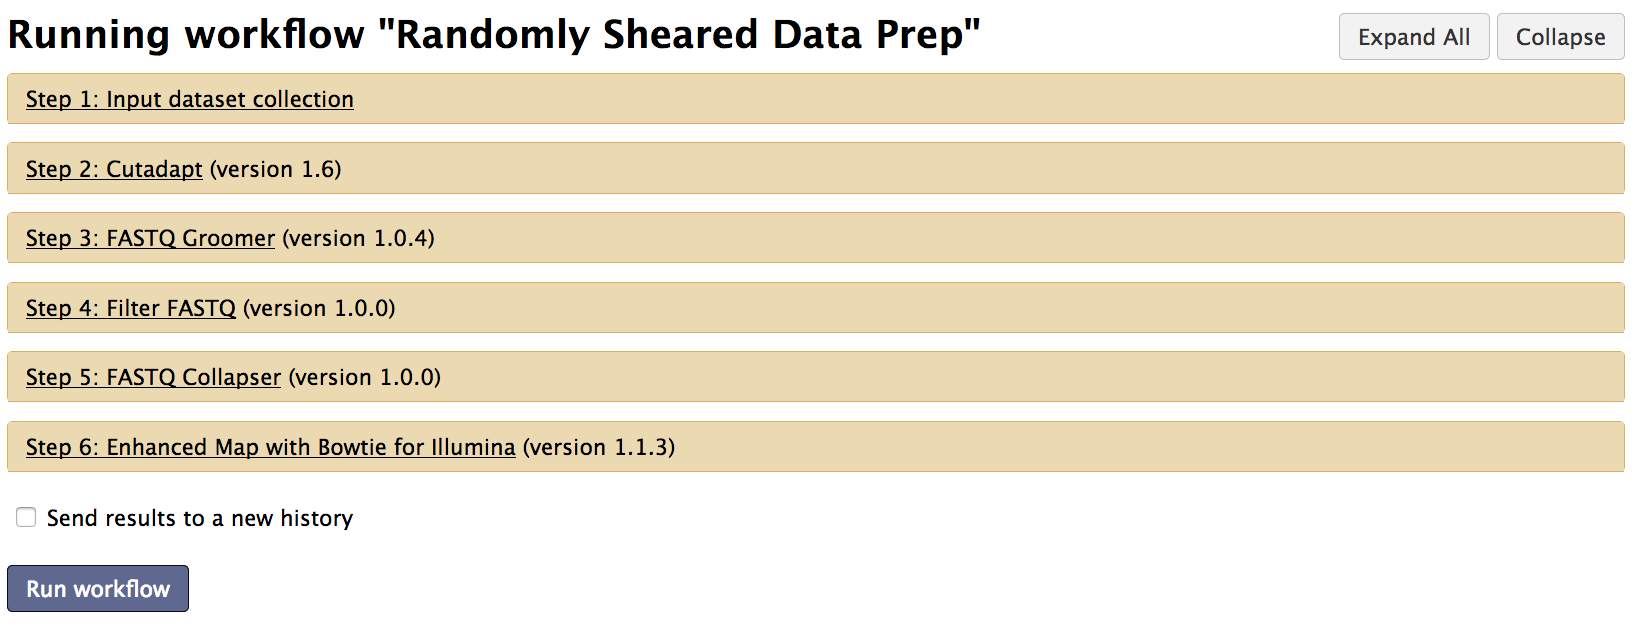
\includegraphics[width=0.8\linewidth]{figs/Random.png}}

\begin{enumerate}
\def\labelenumi{\arabic{enumi}.}
\setcounter{enumi}{2}
\tightlist
\item
  Enter the list of files under ``Step 1: Input dataset collection''
\item
  At ``Step 6: Map with Bowtie for Illumina'', select the fasta genome
  under ``Select the reference genome''. Make sure this is the
  \href{https://en.wikipedia.org/wiki/FASTQ_format}{fasta} file not the
  \href{https://www.ncbi.nlm.nih.gov/Sitemap/samplerecord.html}{genbank}
  file.
\item
  Press ``Run workflow'', and wait for the workflow to finish running
\end{enumerate}

\newpage

\section{Part B: Fitness Analysis}\label{part-b-fitness-analysis}

\subsection{Calculate fitness effect of single mutations and over
annotated
genes}\label{calculate-fitness-effect-of-single-mutations-and-over-annotated-genes}

\href{https://raw.githubusercontent.com/vanOpijnenLab/magenta-p2/blob/master/workflows/Calculate\%20Fitnesses\%20:\%20Aggregate\%20Fitnesses.ga}{Download
Fitness Workflow}

This workflow first calculates fitnesses for each insertion in the
genome, then aggregates them by gene. The aggregate tool can also be
used on multiple Calculate Fitness output files to make a `super'
aggregate file, which calculates fitness of genes by averaging fitness
of all insertions across multiple libraries. Note that this workflow
cannot be run in batch, because each run requires a unique expansion
read, so repeat the below steps for each time 2 condition to be
analyzed.

\begin{enumerate}
\def\labelenumi{\arabic{enumi}.}
\tightlist
\item
  Navigate to the workflow tab, click on the ``Calculate / Aggregate
  Fitness'' workflow, and select ``Run''. A workflow should appear with
  the following steps:
\end{enumerate}

\centerline{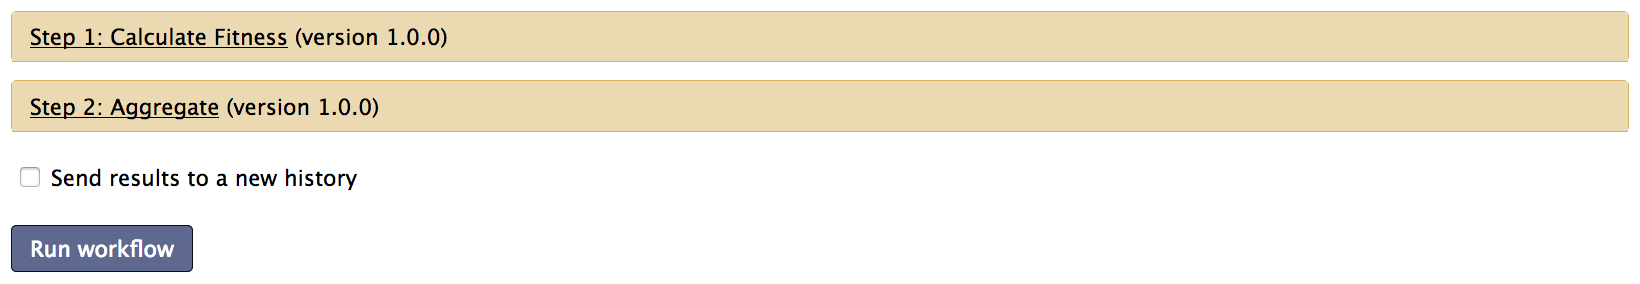
\includegraphics[width=0.8\linewidth]{figs/CalcAgg.png}}

\begin{enumerate}
\def\labelenumi{\arabic{enumi}.}
\setcounter{enumi}{1}
\tightlist
\item
  In ``Step 1: Calculate Fitness'', select the map files from t1, map
  files from t2, GenBank reference genome, and normalization genes under
  the corresponding headers.
\item
  In ``Step 1: Calculate Fitness'', click the edit symbol under
  ``Expansion Factor'' and edit that value with the time 2 sample's
  expansion factor, in that same step.
\item
  In ``Step 2: Aggregate'', Select the GenBank reference genome under
  the corresponding header.
\item
  In ``Step 2: Aggregate'', optionally specify whether to mark certain
  genes (for example, normalization genes, for reference). Choose
  ``Yes'' under ``Mark certain genes?''. Then choose the normalization
  genes file or a similarly formatted file as input.
\item
  Press ``Run workflow'', and wait for the workflow to finish running.
\item
  The output data is from different libraries under the same condition,
  but can be aggregated across gene regions (recommended). Do this by
  navigating to the ``Aggregate'' tool and using the option to ``Insert
  additional CSV fitness files'' as well as selecting ``Yes'' under
  ``Enter a custom blank count?'' as shown below. For the custom blank
  count, simply average the blank counts of each fitness file, which can
  be found in its corresponding calc fitness txt file output. Then enter
  all the fitness files from the same condition, and press ``Execute''!
\end{enumerate}

\subsection{RegionFitness: a non-gene-centric method for discovering
regions important for organismal
fitness}\label{regionfitness-a-non-gene-centric-method-for-discovering-regions-important-for-organismal-fitness}

The method for calculating the aggregate fitness value of a gene relies
on the genomic start and end coordinates of the region, which is
retrievable from the organism's Genbank record. However, not all
official genome records are complete or well annotated beyond genes. At
the same time, it has been shown that non-coding RNAs have an important
role in virulence and other functions. Therefore, to enable discovery of
such regions that may have an important fitness value to the organism,
this tools uses a sliding window approach to mine Tn-Seq data in a
non-gene-centric manner.

\textbf{Determining window size and step} The entire genome and ordered
Tn-Seq data is scanned by performing assessments of regions at a set
size (base pair length of window) and step (base pairs between the start
of each window). Based on the genome used, typically a window size
between 250 bp and 500 bp is small enough to pick up intergenic regions
or gene domains but large enough to contain enough TA sites and
insertions. However, this can vary depending on organism and insertion
density. The DataOverview tool can help determine these factors.

\textbf{Method} In each regional profile, the aggregate fitness cost for
insertions and the insertion representation in that region is
calculated. To assess insertion representation, we follow the method
used by Zhang et. al.14. For a given region, with x insertions and n TA
sites, 10,000 random sets of n TA sites are selected and the average of
insertions over TA sites is calculated for each. The 10,000 resulting
means create a null distribution. The p-value can be derived for the
original region of interest by ranking it on the distribution for x/n. A
statistically underrepresented number of insertions for a region will be
significant if the p-value is below the critical value. Gene annotations
are also recorded if they are contained in the region. In the future, a
function to identify promoter regions based on -10 and -35 box sequences
and domain regions will be useful.

SlidingWindow performs the fitness and insertion representation
assessments in approximately 8 minutes for a two-thousand base pair
genome with \textasciitilde{}70\% TA site saturation. For the Tn-Seq
data from two strains of Streptococcus pneumoniae grown in two
conditions, 211,151 regions (300 bp) across the 2,112,148 bp genome were
profiled using this approach and later used for comparative analyses.

\centerline{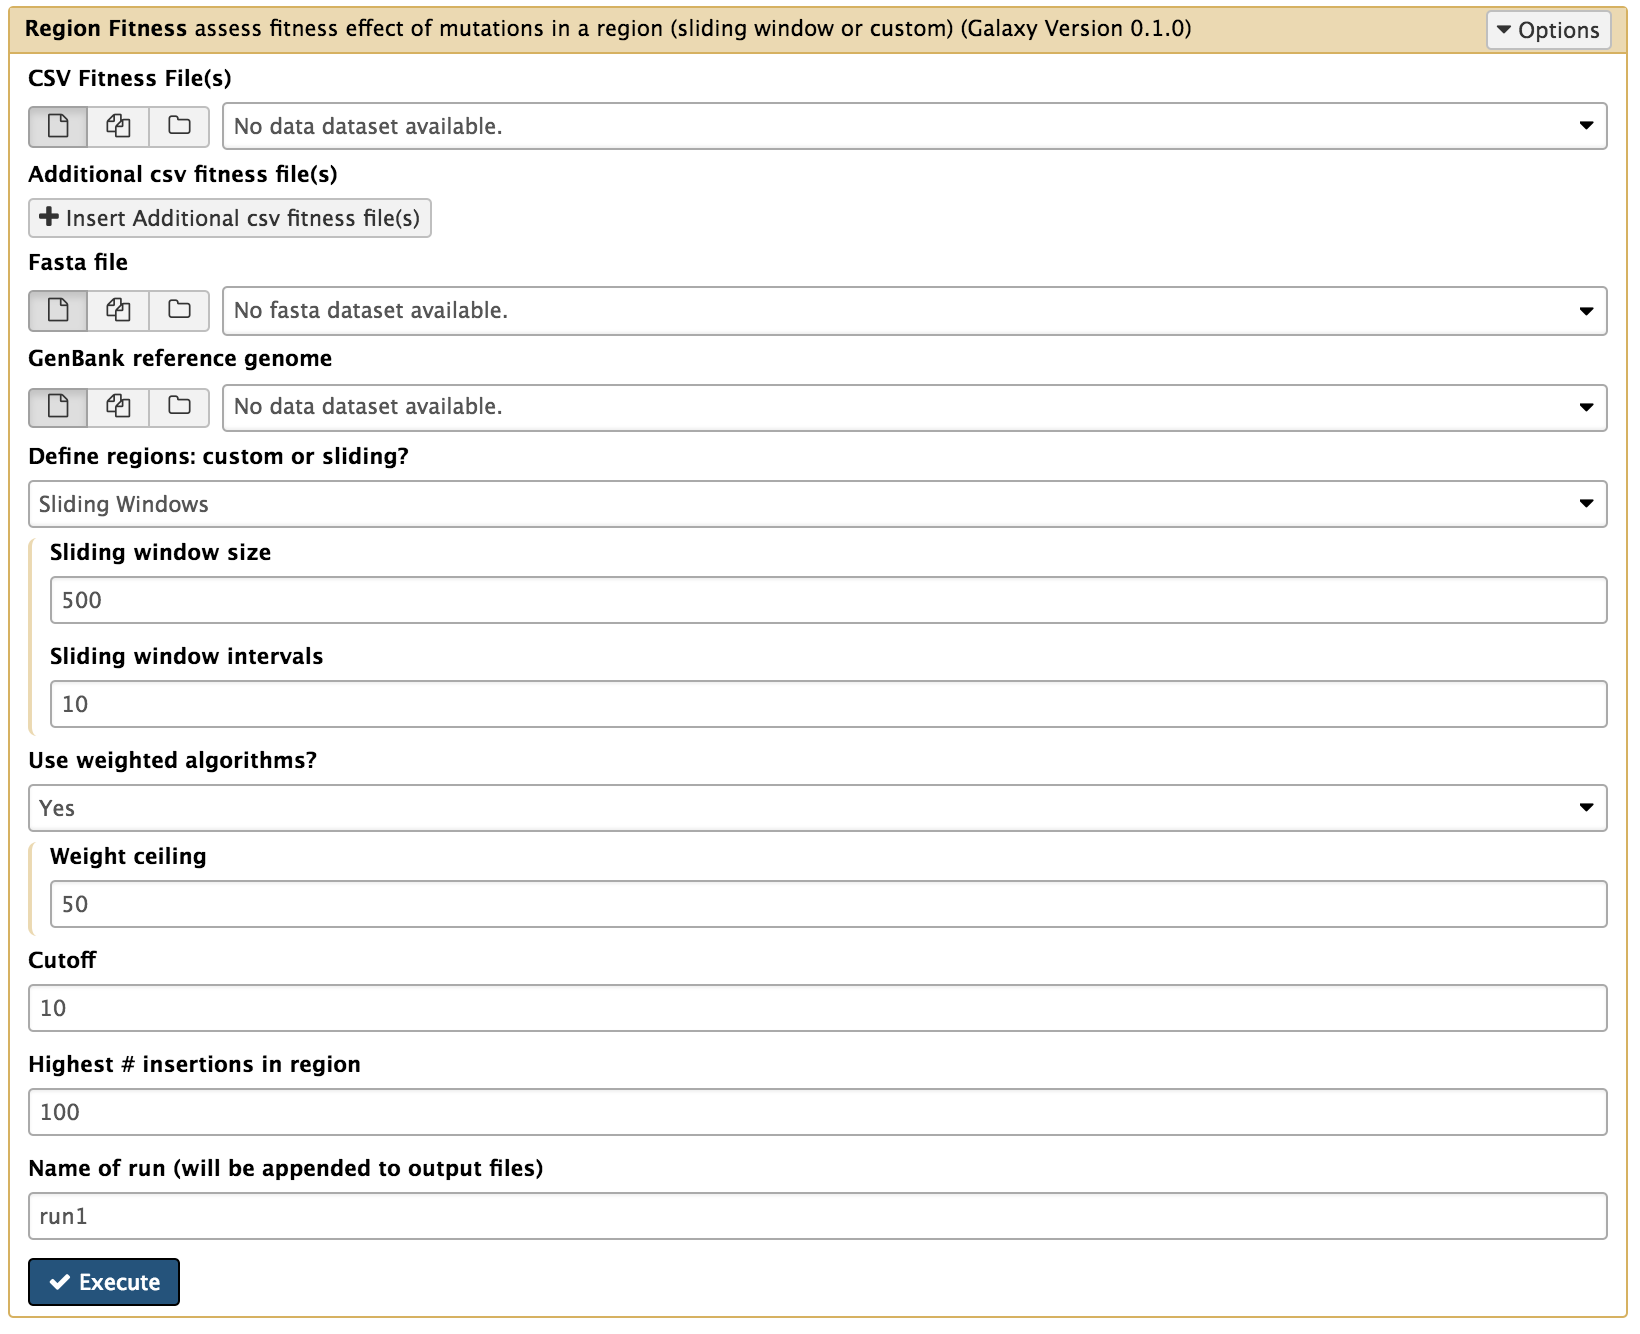
\includegraphics[width=0.8\linewidth]{figs/regionFitness_galaxy.png}}

\newpage

\section{Part C: Comparative
Analyses}\label{part-c-comparative-analyses}

\textbf{Table 1. A summary of analsyis tools in MAGenTA.}

\begin{longtable}[]{@{}lll@{}}
\toprule
\begin{minipage}[b]{0.13\columnwidth}\raggedright\strut
Tool\strut
\end{minipage} & \begin{minipage}[b]{0.40\columnwidth}\raggedright\strut
Function\strut
\end{minipage} & \begin{minipage}[b]{0.38\columnwidth}\raggedright\strut
Research Questions Addressed\strut
\end{minipage}\tabularnewline
\midrule
\endhead
\begin{minipage}[t]{0.13\columnwidth}\raggedright\strut
DataOverview\strut
\end{minipage} & \begin{minipage}[t]{0.40\columnwidth}\raggedright\strut
Produces a summary file of information about TA sites and insertions in
the genome, libraries, and gene/intergenic regions\strut
\end{minipage} & \begin{minipage}[t]{0.38\columnwidth}\raggedright\strut
What is the TA and insertion distribution in the genome for genes and
non-gene regions?\strut
\end{minipage}\tabularnewline
\begin{minipage}[t]{0.13\columnwidth}\raggedright\strut
RegionFitness\strut
\end{minipage} & \begin{minipage}[t]{0.40\columnwidth}\raggedright\strut
Scans the genome data with set window size and step to perform aggregate
fitness and essentiality assessments at each window.\strut
\end{minipage} & \begin{minipage}[t]{0.38\columnwidth}\raggedright\strut
Which unannotated (intergenic or gene domain) regions are important or
essential?\strut
\end{minipage}\tabularnewline
\begin{minipage}[t]{0.13\columnwidth}\raggedright\strut
CustomWindow\strut
\end{minipage} & \begin{minipage}[t]{0.40\columnwidth}\raggedright\strut
Given a list of start and end coordinates, will return aggregate fitness
and essentiality test results. Useful for recalculating info for merged
regions\strut
\end{minipage} & \begin{minipage}[t]{0.38\columnwidth}\raggedright\strut
What is the importance or essentiality of specific regions of
interest?\strut
\end{minipage}\tabularnewline
\begin{minipage}[t]{0.13\columnwidth}\raggedright\strut
CompareGenes\strut
\end{minipage} & \begin{minipage}[t]{0.40\columnwidth}\raggedright\strut
Creates a gene comparison file with significant stats for two Tn-Seq
experiments of the same ref genome. Need aggregate output\strut
\end{minipage} & \begin{minipage}[t]{0.38\columnwidth}\raggedright\strut
How can we compare genes for a given strain in two different conditions?
Which genes are conditionally important?\strut
\end{minipage}\tabularnewline
\begin{minipage}[t]{0.13\columnwidth}\raggedright\strut
CompareStrains\strut
\end{minipage} & \begin{minipage}[t]{0.40\columnwidth}\raggedright\strut
Creates a gene comparison file with significant stats for two Tn-Seq
experiments of different strains (genomes). Need conversion file and
aggregate output.\strut
\end{minipage} & \begin{minipage}[t]{0.38\columnwidth}\raggedright\strut
How can we compare homologous genes for two strains? Which genes have a
strain-dependent importance?\strut
\end{minipage}\tabularnewline
\begin{minipage}[t]{0.13\columnwidth}\raggedright\strut
CompareRegions\strut
\end{minipage} & \begin{minipage}[t]{0.40\columnwidth}\raggedright\strut
Creates a comparison file with significance statistics for two Tn-Seq
experiments of different strains (genomes). Need sliding window
output\strut
\end{minipage} & \begin{minipage}[t]{0.38\columnwidth}\raggedright\strut
How can we compare intergenic or gene domain regions for the same strain
in two conditions?\strut
\end{minipage}\tabularnewline
\bottomrule
\end{longtable}

\subsection{DataOverview: Characterizing the reference genome and
genome-wide insertion
data}\label{dataoverview-characterizing-the-reference-genome-and-genome-wide-insertion-data}

Prior to Tn-seq data analysis it is important to understand the
genome-wide scale and context of the data. Large differences in
sequencing coverage, insertion representation, and GC content between
genomes can affect the robustness of the comparative analyses performed
by MAGenTA. Tn-Seq is also generally performed with replicate libraries,
where differences (if they exist) would be important to know. The
DataOverview tool produces a summary of genome-wide insertion
representation and inherent genome characteristics. The input data are
queried for TA sites and insertions with respect to

\begin{enumerate}
\def\labelenumi{\arabic{enumi}.}
\tightlist
\item
  The genome
\item
  Open reading frames denoted by start and stop codons
\item
  Annotated genes from the Genbank record
\item
  Intergenic regions
\end{enumerate}

\centerline{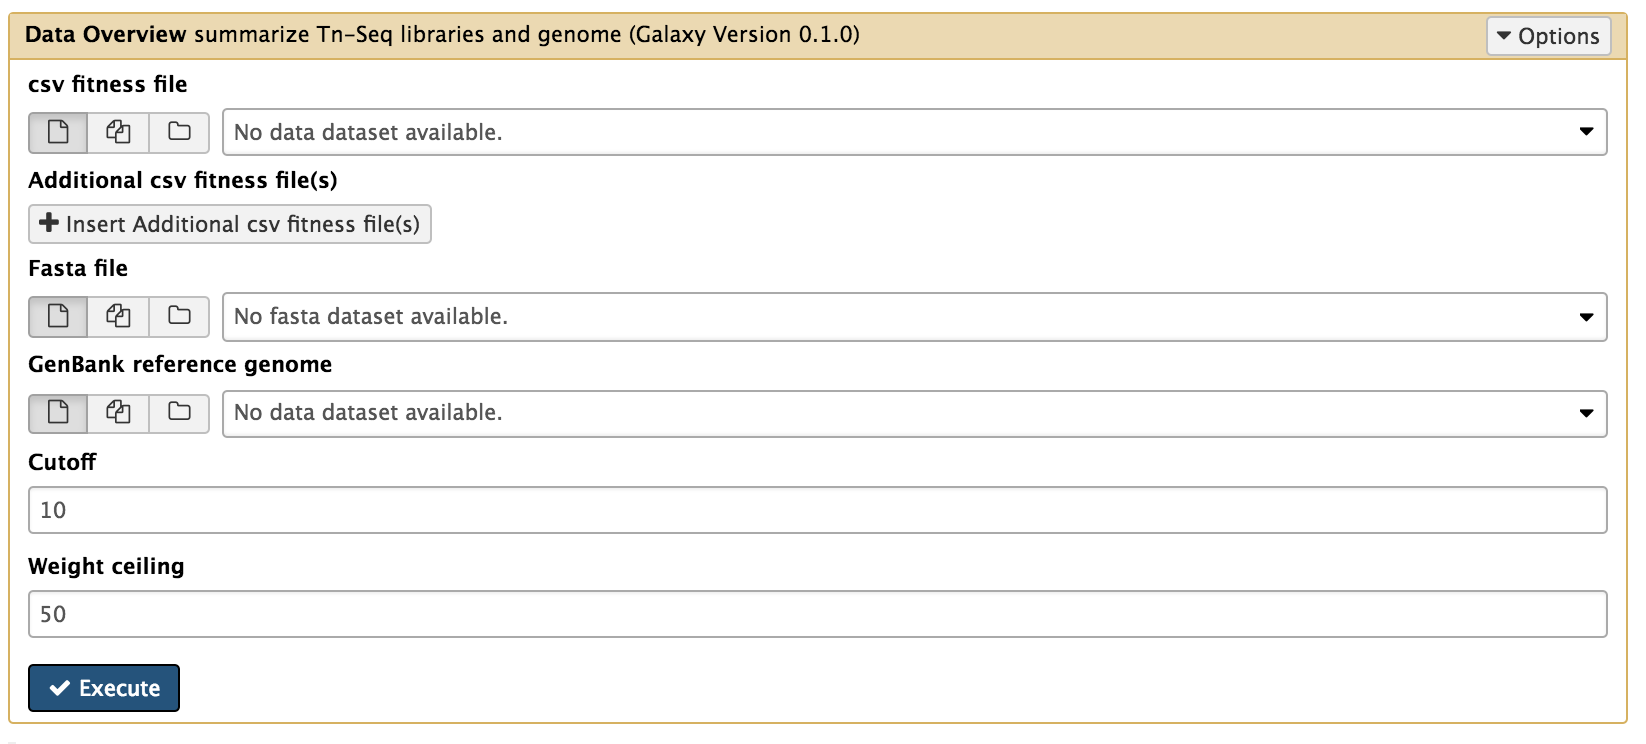
\includegraphics[width=0.8\linewidth]{figs/dataOverview_galaxy.png}}

\textbf{Sample Output}

\textbf{Table 2. The DataOverview tool outputs genome and Tn-Seq related
summary information.} The summary includes genome and gene-wide
insertion representation for each library, including how many insertions
would be filtered out given a cutoff requirement for the number of reads
representing each insertion.

\begin{longtable}[]{@{}lll@{}}
\toprule
\begin{minipage}[b]{0.32\columnwidth}\raggedright\strut
\strut
\end{minipage} & \begin{minipage}[b]{0.32\columnwidth}\raggedright\strut
Strain1\strut
\end{minipage} & \begin{minipage}[b]{0.32\columnwidth}\raggedright\strut
Strain2\strut
\end{minipage}\tabularnewline
\midrule
\endhead
Genbank Record & NC\_003028 & NC\_0012469\tabularnewline
Genome Size (bp) & 2160842 & 2112148\tabularnewline
GC content & 39.70\% & 39.77\%\tabularnewline
Number of Genes & 2390 & 2204\tabularnewline
Total number of TA sites & 141459 & 137693\tabularnewline
Genome coverage by TA sites & 6.55\% & 6.52\%\tabularnewline
Largest gap between TA sites (bp) & 252 & 206\tabularnewline
Genome coverage by insertions & 1.33\% & 3.68\%\tabularnewline
TA site coverage by insertions & 32.80\% & 73.12\%\tabularnewline
TA site coverage by filtered insertions* & 20.28\% &
56.45\%\tabularnewline
Largest gap between insertions (bp) & 14996 & 6708\tabularnewline
Smallest ORF (bp) & 6 & 6\tabularnewline
Largest ORF (bp) & 220 & 220\tabularnewline
Max number TA sites in an ORF & 10 & 10\tabularnewline
Number of ORFs without TA sites & 6997 & 6701\tabularnewline
Average gene length & 803 & 834\tabularnewline
Minimum gene length & 30 & 65\tabularnewline
Max gene length & 14330 & 6701\tabularnewline
Average insertions in a gene & 9.84 & 28.4\tabularnewline
Minimum insertions in a gene & 0 & 0\tabularnewline
Maximum insertions in a gene & 237 & 420\tabularnewline
Genes with insertions & 65\% & 77\%\tabularnewline
Number of genes without insertions & 564 & 257\tabularnewline
Insertions outside of annotated genes & 15773 & 43266\tabularnewline
Insertions in intergenic regions** & 54.98\% & 55.66\%\tabularnewline
\bottomrule
\end{longtable}

\subsection{CompareGenes: Comparative gene analysis for the same
organism}\label{comparegenes-comparative-gene-analysis-for-the-same-organism}

Comparative gene analysis for two experiments of the same organism
(i.e.~One strain tested in Glucose and in Glucose+Antibiotic) involves
merging two output files from the fitness script, then performing a
t-test and calculating average fitness difference for each gene. This
process can be performed in a spreadsheet applciation, such as Excel.
However, GeneCompare can perform it in less than five seconds for 2000
gene.

\centerline{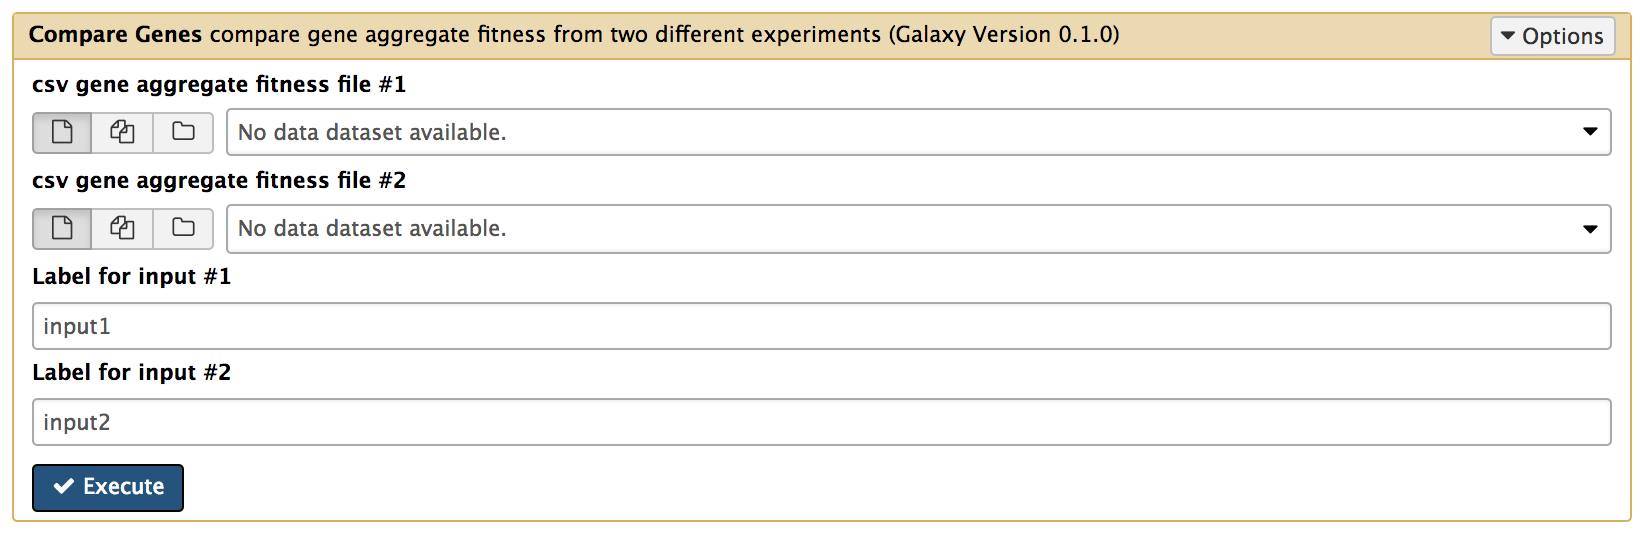
\includegraphics[width=0.8\linewidth]{figs/compareGenes_galaxy.png}}

\subsection{CompareStrain: Comparative gene analysis for different
organisms}\label{comparestrain-comparative-gene-analysis-for-different-organisms}

The CompareStrain tool, a variation of GeneCompare, is specifically for
gene comparisons across two experiments from different
organisms/strains. Since gene identification numbers will be different
at the organism/strain level, a file containing the homologous genes is
required. The same output as GeneCompare will be produced and can be
used in downstream analysis tools. An automated method for extracting
homologous genes will be a useful future improvement to this tool.

\subsection{CompareRegions: Comparative analysis of small, unannotated
regions}\label{compareregions-comparative-analysis-of-small-unannotated-regions}

CompareRegions takes results from the RegionFitness tool and performs a
similar comparative analysis as done on genes by GeneCompare and
StrainCompare for genes. Since start and end coordinates define windows
(or regions), only comparisons between datasets from the same organism
(same genome) can be performed.

In the example shown, over 200,000 300-bp windows for Tn-Seq data from
Taiwan-19F grown in glucose and the presence of daptomycin are assessed
for conditionally important regions using the adjusted p-value (FDR) and
fitness difference between the two conditions. As shown in the yellow
highlighted area, 583 regions met the criteria for having adjusted
p-values below a critical value of 0.01 and a fitness difference greater
than 0.1. Distributions of regions in 20 unique genes and two intergenic
regions are shown in the table.

\centerline{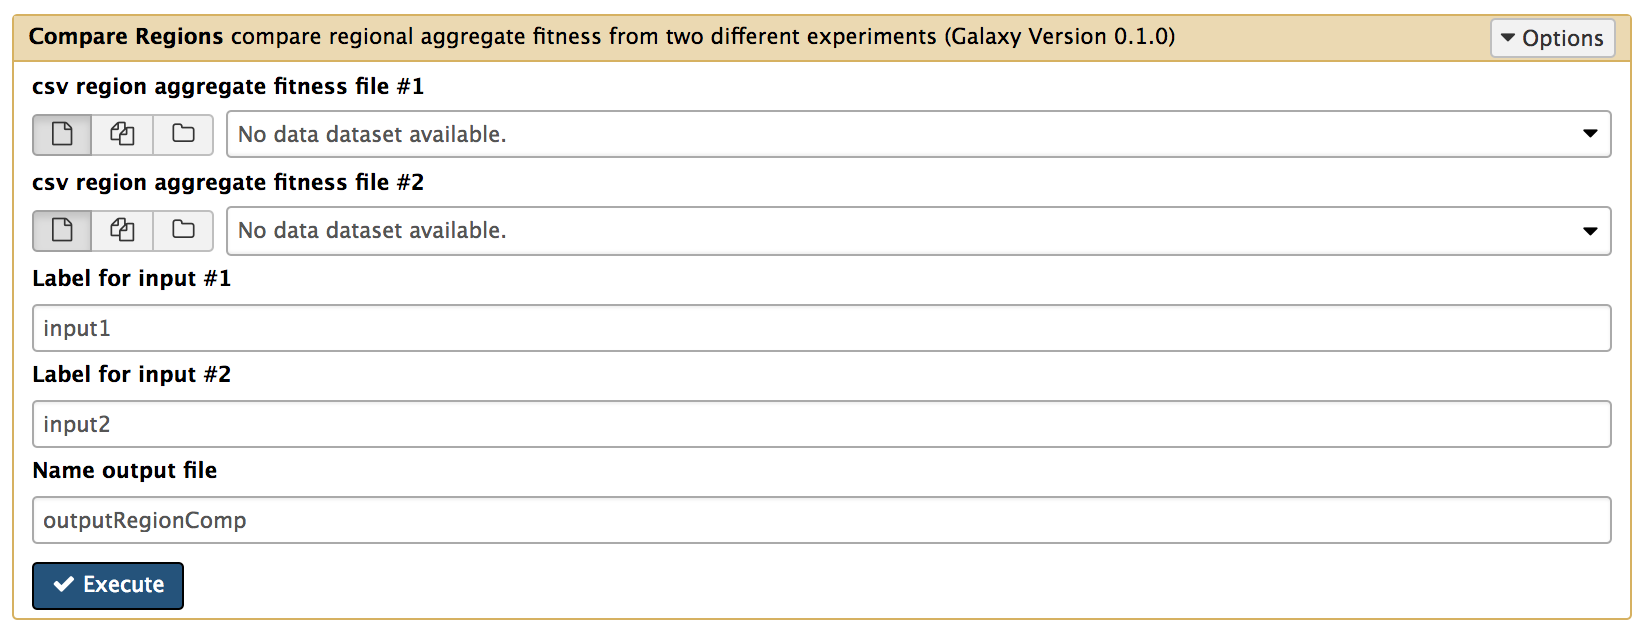
\includegraphics[width=0.8\linewidth]{figs/compareRegions_galaxy.png}}

\subsection{SingleFitness: aggregate fitness information across multiple
libraries for one weighted fitness value per insertion
mutant}\label{singlefitness-aggregate-fitness-information-across-multiple-libraries-for-one-weighted-fitness-value-per-insertion-mutant}

\centerline{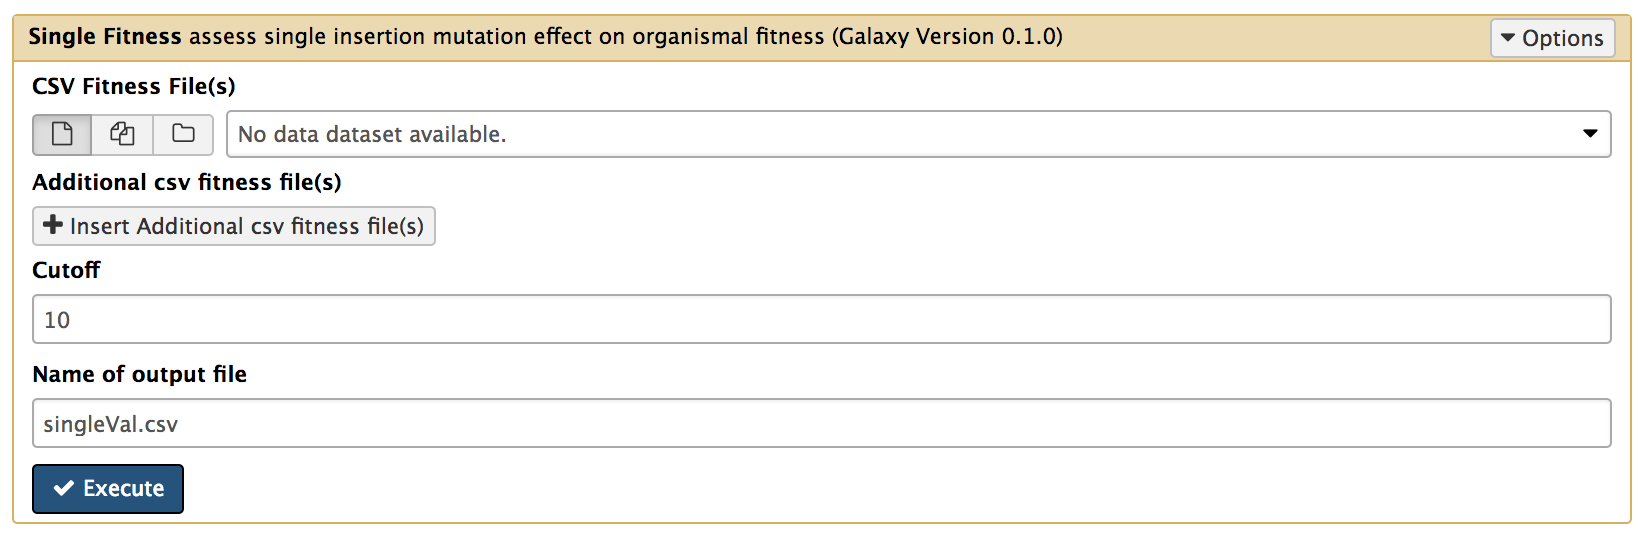
\includegraphics[width=0.8\linewidth]{figs/singleFitness_galaxy.png}}

\section{Performing Data pre-processing and MAGenTA analyses on the
Command-line}\label{performing-data-pre-processing-and-magenta-analyses-on-the-command-line}

\subsection{Data Prep: Fastx Toolkit and
Bowtie}\label{data-prep-fastx-toolkit-and-bowtie}

\begin{enumerate}
\def\labelenumi{\arabic{enumi}.}
\tightlist
\item
  Download and install the
  \href{http://hannonlab.cshl.edu/fastx_toolkit/}{FASTX Toolkit} and
  \href{http://bowtie-bio.sourceforge.net/index.shtml}{Bowtie}. For more
  on the usage of the fastx\_toolkit see its
  \href{http://hannonlab.cshl.edu/fastx_toolkit/commandline.html}{manual},
  and for more on Bowtie see its
  \href{http://bowtie-bio.sourceforge.net/manual.shtml}{manual}.
\item
  Split data by experimental condition (i.e.~barcodes) with fastx
  barcode splitter and remove all non-genomic DNA (e.g.~barcodes) with
  fastx trimmer. These steps may be done in whatever order best suits
  the data.
\item
  Filter reads by quality (e.g.~a minimum quality of 8) using fastq
  quality filter.
\item
  Collapse reads using fastq collapser.
\item
  Map reads using Bowtie. We recommend using the following flags: -n 1
  (maximum 1 mismatch) --best (Wwether or not to make Bowtie guarantee
  that reported singleton alignments are `best' in terms of stratum and
  quality) -y (try hard) and -m 1 (supress all alignments if more than
  one can be found)
\end{enumerate}

\subsection{Downloading command-line
tools}\label{downloading-command-line-tools}

Command-line tools for MAGenTA are open source and available through
GitHub

\begin{verbatim}
git clone https://github.com/vanOpijnenLab/magenta-p2.git
\end{verbatim}

Or \href{https://github.com/vanOpijnenLab/magenta-p2}{download the
MAGenTA project repository}

\subsection{Script Usage}\label{script-usage}

\subsubsection{CalculateFitness: calculate fitness of single insertion
mutants using read counts at two time
points}\label{calculatefitness-calculate-fitness-of-single-insertion-mutants-using-read-counts-at-two-time-points}

\paragraph{Usage}\label{usage}

\begin{verbatim}
python calc_fitness.py <options>
\end{verbatim}

\paragraph{Required Inputs}\label{required-inputs}

\begin{longtable}[]{@{}ll@{}}
\toprule
Flag & Description\tabularnewline
\midrule
\endhead
ref & The name of the reference genome file, in GenBank
format\tabularnewline
t1 & The name of the bowtie mapfile from time point 1\tabularnewline
t2 & The name of the bowtie mapfile from time point 2\tabularnewline
out & Name of a file to enter the .csv output\tabularnewline
\bottomrule
\end{longtable}

\paragraph{Optional Inputs}\label{optional-inputs}

\begin{longtable}[]{@{}ll@{}}
\toprule
\begin{minipage}[b]{0.08\columnwidth}\raggedright\strut
Flag\strut
\end{minipage} & \begin{minipage}[b]{0.86\columnwidth}\raggedright\strut
Description\strut
\end{minipage}\tabularnewline
\midrule
\endhead
\begin{minipage}[t]{0.08\columnwidth}\raggedright\strut
expansion\strut
\end{minipage} & \begin{minipage}[t]{0.86\columnwidth}\raggedright\strut
Expansion factor (default: 250)\strut
\end{minipage}\tabularnewline
\begin{minipage}[t]{0.08\columnwidth}\raggedright\strut
reads1\strut
\end{minipage} & \begin{minipage}[t]{0.86\columnwidth}\raggedright\strut
The number of reads to be used to calculate the correction factor for
time 0 (default counted from bowtie output)\strut
\end{minipage}\tabularnewline
\begin{minipage}[t]{0.08\columnwidth}\raggedright\strut
reads2\strut
\end{minipage} & \begin{minipage}[t]{0.86\columnwidth}\raggedright\strut
The number of reads to be used to calculate the correction factor for
time 1 (default counted from bowtie output)\strut
\end{minipage}\tabularnewline
\begin{minipage}[t]{0.08\columnwidth}\raggedright\strut
cutoff1\strut
\end{minipage} & \begin{minipage}[t]{0.86\columnwidth}\raggedright\strut
Discard any positions where the average of counted transcripts at time 0
and time 1 is below this number (default 0)\strut
\end{minipage}\tabularnewline
\begin{minipage}[t]{0.08\columnwidth}\raggedright\strut
cutoff2\strut
\end{minipage} & \begin{minipage}[t]{0.86\columnwidth}\raggedright\strut
Discard any positions within the normalization genes where the average
of counted transcripts at time 0 and time 1 is below this number
(default 10)\strut
\end{minipage}\tabularnewline
\begin{minipage}[t]{0.08\columnwidth}\raggedright\strut
strand\strut
\end{minipage} & \begin{minipage}[t]{0.86\columnwidth}\raggedright\strut
Use only the specified strand ( + or -) when counting transcripts
(default: both)\strut
\end{minipage}\tabularnewline
\begin{minipage}[t]{0.08\columnwidth}\raggedright\strut
normalize\strut
\end{minipage} & \begin{minipage}[t]{0.86\columnwidth}\raggedright\strut
A file that contains a list of genes that should have a fitness of 1 -
used for normalization and bottleneck calculations.\strut
\end{minipage}\tabularnewline
\begin{minipage}[t]{0.08\columnwidth}\raggedright\strut
b\strut
\end{minipage} & \begin{minipage}[t]{0.86\columnwidth}\raggedright\strut
Calculate bottleneck value (the percentage of insertions randomly lost)
from all genes (rather than only normalization genes\strut
\end{minipage}\tabularnewline
\begin{minipage}[t]{0.08\columnwidth}\raggedright\strut
maxweight\strut
\end{minipage} & \begin{minipage}[t]{0.86\columnwidth}\raggedright\strut
The maximum weight a transposon gene can have in normalization
calculations\strut
\end{minipage}\tabularnewline
\begin{minipage}[t]{0.08\columnwidth}\raggedright\strut
multiply\strut
\end{minipage} & \begin{minipage}[t]{0.86\columnwidth}\raggedright\strut
Multiply all fitness scores by a certain value (e.g., the fitness of a
knockout).\strut
\end{minipage}\tabularnewline
\begin{minipage}[t]{0.08\columnwidth}\raggedright\strut
ef\strut
\end{minipage} & \begin{minipage}[t]{0.86\columnwidth}\raggedright\strut
Exclude insertions that occur in the first N amount (\%) of gene becuase
may not affect gene function.\strut
\end{minipage}\tabularnewline
\begin{minipage}[t]{0.08\columnwidth}\raggedright\strut
el\strut
\end{minipage} & \begin{minipage}[t]{0.86\columnwidth}\raggedright\strut
Exclude insertions in the last N amount (\%) of the gene--considering
truncation may not affect gene function.\strut
\end{minipage}\tabularnewline
\begin{minipage}[t]{0.08\columnwidth}\raggedright\strut
wig\strut
\end{minipage} & \begin{minipage}[t]{0.86\columnwidth}\raggedright\strut
Create a wiggle file for viewing in a genome browser. Provide a
filename.\strut
\end{minipage}\tabularnewline
\begin{minipage}[t]{0.08\columnwidth}\raggedright\strut
uncol\strut
\end{minipage} & \begin{minipage}[t]{0.86\columnwidth}\raggedright\strut
Use if reads were uncollapsed when mapped.\strut
\end{minipage}\tabularnewline
\bottomrule
\end{longtable}

\subsubsection{AggregateFitness: calculate aggregate fitness cost over
genes}\label{aggregatefitness-calculate-aggregate-fitness-cost-over-genes}

\paragraph{Usage}\label{usage-1}

\begin{verbatim}
python aggregate.py -o <output file> <options> <inputs or -d directory>
\end{verbatim}

\paragraph{Required Inputs}\label{required-inputs-1}

\begin{longtable}[]{@{}ll@{}}
\toprule
Flag & Description\tabularnewline
\midrule
\endhead
o & Output file for aggregated data\tabularnewline
\bottomrule
\end{longtable}

\paragraph{Optional Inputs}\label{optional-inputs-1}

\begin{longtable}[]{@{}ll@{}}
\toprule
\begin{minipage}[b]{0.06\columnwidth}\raggedright\strut
Flag\strut
\end{minipage} & \begin{minipage}[b]{0.88\columnwidth}\raggedright\strut
Description\strut
\end{minipage}\tabularnewline
\midrule
\endhead
\begin{minipage}[t]{0.06\columnwidth}\raggedright\strut
c\strut
\end{minipage} & \begin{minipage}[t]{0.88\columnwidth}\raggedright\strut
Check for missing genes in the data set - provide a reference genome in
genbank format. Missing genes will be sent to stdout\strut
\end{minipage}\tabularnewline
\begin{minipage}[t]{0.06\columnwidth}\raggedright\strut
m\strut
\end{minipage} & \begin{minipage}[t]{0.88\columnwidth}\raggedright\strut
Place a mark in an extra column for this set of genes. Provide a file
with a list of genes seperated by newlines\strut
\end{minipage}\tabularnewline
\begin{minipage}[t]{0.06\columnwidth}\raggedright\strut
x\strut
\end{minipage} & \begin{minipage}[t]{0.88\columnwidth}\raggedright\strut
Cutoff: Don't include fitness scores with average counts (c1+c2)/2
\textless{} x (default: 10)\strut
\end{minipage}\tabularnewline
\begin{minipage}[t]{0.06\columnwidth}\raggedright\strut
b\strut
\end{minipage} & \begin{minipage}[t]{0.88\columnwidth}\raggedright\strut
Bottleneck value: The percentage of insertions randomly lost, which will
be discounted for all genes (for example, 20\% would be entered as 0.20;
default 0.0)\strut
\end{minipage}\tabularnewline
\begin{minipage}[t]{0.06\columnwidth}\raggedright\strut
f\strut
\end{minipage} & \begin{minipage}[t]{0.88\columnwidth}\raggedright\strut
An in-between file carrying information on the blank count found from
calc\_fitness or consol\_fitness, one of two ways to pass a blank count
to this script\strut
\end{minipage}\tabularnewline
\begin{minipage}[t]{0.06\columnwidth}\raggedright\strut
w\strut
\end{minipage} & \begin{minipage}[t]{0.88\columnwidth}\raggedright\strut
Use weighted algorithm in calculations\strut
\end{minipage}\tabularnewline
\begin{minipage}[t]{0.06\columnwidth}\raggedright\strut
l\strut
\end{minipage} & \begin{minipage}[t]{0.88\columnwidth}\raggedright\strut
Weight ceiling: maximum value to use as a weight (default:
999,999)\strut
\end{minipage}\tabularnewline
\bottomrule
\end{longtable}

\subsubsection{DataOverview}\label{dataoverview}

\paragraph{Usage}\label{usage-2}

\begin{verbatim}
perl dataOverview.pl <otpions> <inputs or -d directory>
\end{verbatim}

\paragraph{Required Inputs}\label{required-inputs-2}

\begin{longtable}[]{@{}ll@{}}
\toprule
\begin{minipage}[b]{0.05\columnwidth}\raggedright\strut
Flag\strut
\end{minipage} & \begin{minipage}[b]{0.89\columnwidth}\raggedright\strut
Description\strut
\end{minipage}\tabularnewline
\midrule
\endhead
\begin{minipage}[t]{0.05\columnwidth}\raggedright\strut
d\strut
\end{minipage} & \begin{minipage}[t]{0.89\columnwidth}\raggedright\strut
Directory containing all input files (output files from calcFitness
tool) OR In the command line (without a flag) input filename(s)\strut
\end{minipage}\tabularnewline
\begin{minipage}[t]{0.05\columnwidth}\raggedright\strut
f\strut
\end{minipage} & \begin{minipage}[t]{0.89\columnwidth}\raggedright\strut
Filename for genome sequence in fasta format\strut
\end{minipage}\tabularnewline
\begin{minipage}[t]{0.05\columnwidth}\raggedright\strut
r\strut
\end{minipage} & \begin{minipage}[t]{0.89\columnwidth}\raggedright\strut
Filename for genome annotation in GenBank format\strut
\end{minipage}\tabularnewline
\bottomrule
\end{longtable}

\paragraph{Optional Inputs}\label{optional-inputs-2}

\begin{longtable}[]{@{}ll@{}}
\toprule
Flag & Description\tabularnewline
\midrule
\endhead
h & Print usage\tabularnewline
o & Filename for output. Default: standard output\tabularnewline
c & Cutoff average(c1+c2)\textgreater{}c. Default: 15\tabularnewline
\bottomrule
\end{longtable}

\subsubsection{GeneCompare: Comparative gene analysis for the same
organism}\label{genecompare-comparative-gene-analysis-for-the-same-organism}

Comparative gene analysis for two experiments of the same organism
(i.e.~One strain tested in Glucose and in Glucose+Antibiotic) involves
merging two output files from the fitness script, then performing a
t-test and calculating average fitness difference for each gene. This
process can be performed in a spreadsheet applciation, such as Excel.
However, GeneCompare can perform it in less than five seconds for 2000
gene.

\paragraph{Usage}\label{usage-3}

\begin{verbatim}
perl compGenes.pl <options> <inputs or -d directory>
\end{verbatim}

\paragraph{Required Inputs}\label{required-inputs-3}

\begin{longtable}[]{@{}ll@{}}
\toprule
\begin{minipage}[b]{0.05\columnwidth}\raggedright\strut
Flag\strut
\end{minipage} & \begin{minipage}[b]{0.89\columnwidth}\raggedright\strut
Description\strut
\end{minipage}\tabularnewline
\midrule
\endhead
\begin{minipage}[t]{0.05\columnwidth}\raggedright\strut
d\strut
\end{minipage} & \begin{minipage}[t]{0.89\columnwidth}\raggedright\strut
Directory containing all input files (output files from calcFitness
tool) OR In the command line (without a flag) input filename(s)\strut
\end{minipage}\tabularnewline
\begin{minipage}[t]{0.05\columnwidth}\raggedright\strut
c\strut
\end{minipage} & \begin{minipage}[t]{0.89\columnwidth}\raggedright\strut
Tab delimited file with homologous genes, one gene homolog pair per
line\strut
\end{minipage}\tabularnewline
\bottomrule
\end{longtable}

\paragraph{Optional Inputs}\label{optional-inputs-3}

\begin{longtable}[]{@{}ll@{}}
\toprule
\begin{minipage}[b]{0.06\columnwidth}\raggedright\strut
Flag\strut
\end{minipage} & \begin{minipage}[b]{0.88\columnwidth}\raggedright\strut
Description\strut
\end{minipage}\tabularnewline
\midrule
\endhead
\begin{minipage}[t]{0.06\columnwidth}\raggedright\strut
h\strut
\end{minipage} & \begin{minipage}[t]{0.88\columnwidth}\raggedright\strut
Print usage\strut
\end{minipage}\tabularnewline
\begin{minipage}[t]{0.06\columnwidth}\raggedright\strut
o\strut
\end{minipage} & \begin{minipage}[t]{0.88\columnwidth}\raggedright\strut
Filename for output. Default: compFile1File2.csv\strut
\end{minipage}\tabularnewline
\begin{minipage}[t]{0.06\columnwidth}\raggedright\strut
l\strut
\end{minipage} & \begin{minipage}[t]{0.88\columnwidth}\raggedright\strut
Labels for input files. Two strings, comma separated (i.e. -l
expt1,expt2). Order should match file order. Default: input
filenames.\strut
\end{minipage}\tabularnewline
\bottomrule
\end{longtable}

\subsubsection{StrainCompare: Comparative gene analysis for different
organisms}\label{straincompare-comparative-gene-analysis-for-different-organisms}

The StrainCompare tool, a variation of GeneCompare, is specifically for
gene comparisons across two experiments from different
organisms/strains. Since gene identification numbers will be different
at the organism/strain level, a file containing the homologous genes is
required. The same output as GeneCompare will be produced and can be
used in downstream analysis tools. An automated method for extracting
homologous genes will be a useful future improvement to this tool.

\paragraph{Usage}\label{usage-4}

\begin{verbatim}
perl compStrains.pl <options> <inputs or -d directory>
\end{verbatim}

\paragraph{Required Inputs}\label{required-inputs-4}

\begin{longtable}[]{@{}ll@{}}
\toprule
\begin{minipage}[b]{0.05\columnwidth}\raggedright\strut
Flag\strut
\end{minipage} & \begin{minipage}[b]{0.89\columnwidth}\raggedright\strut
Description\strut
\end{minipage}\tabularnewline
\midrule
\endhead
\begin{minipage}[t]{0.05\columnwidth}\raggedright\strut
d\strut
\end{minipage} & \begin{minipage}[t]{0.89\columnwidth}\raggedright\strut
Directory containing all input files (output files from calcFitness
tool) OR In the command line (without a flag) input filename(s)\strut
\end{minipage}\tabularnewline
\begin{minipage}[t]{0.05\columnwidth}\raggedright\strut
c\strut
\end{minipage} & \begin{minipage}[t]{0.89\columnwidth}\raggedright\strut
Tab delimited file with homologous genes, one gene homolog pair per
line\strut
\end{minipage}\tabularnewline
\bottomrule
\end{longtable}

\paragraph{Optional Inputs}\label{optional-inputs-4}

\begin{longtable}[]{@{}ll@{}}
\toprule
\begin{minipage}[b]{0.06\columnwidth}\raggedright\strut
Flag\strut
\end{minipage} & \begin{minipage}[b]{0.88\columnwidth}\raggedright\strut
Description\strut
\end{minipage}\tabularnewline
\midrule
\endhead
\begin{minipage}[t]{0.06\columnwidth}\raggedright\strut
h\strut
\end{minipage} & \begin{minipage}[t]{0.88\columnwidth}\raggedright\strut
Print usage\strut
\end{minipage}\tabularnewline
\begin{minipage}[t]{0.06\columnwidth}\raggedright\strut
o\strut
\end{minipage} & \begin{minipage}[t]{0.88\columnwidth}\raggedright\strut
Filename for output. Default: compFile1File2.csv\strut
\end{minipage}\tabularnewline
\begin{minipage}[t]{0.06\columnwidth}\raggedright\strut
l\strut
\end{minipage} & \begin{minipage}[t]{0.88\columnwidth}\raggedright\strut
Labels for input files. Two strings, comma separated (i.e. -l
expt1,expt2). Order should match file order. Default: input
filenames.\strut
\end{minipage}\tabularnewline
\bottomrule
\end{longtable}

\subsubsection{Region Fitness}\label{region-fitness}

\paragraph{Usage}\label{usage-5}

\begin{verbatim}
perl slidingWindow.pl <options> <inputs or -d directory>
\end{verbatim}

\paragraph{Required Inputs}\label{required-inputs-5}

\begin{longtable}[]{@{}ll@{}}
\toprule
\begin{minipage}[b]{0.05\columnwidth}\raggedright\strut
Flag\strut
\end{minipage} & \begin{minipage}[b]{0.89\columnwidth}\raggedright\strut
Description\strut
\end{minipage}\tabularnewline
\midrule
\endhead
\begin{minipage}[t]{0.05\columnwidth}\raggedright\strut
d\strut
\end{minipage} & \begin{minipage}[t]{0.89\columnwidth}\raggedright\strut
Directory containing all input files (output files from calcFitness
tool) OR In the command line (without a flag) input filename(s)\strut
\end{minipage}\tabularnewline
\begin{minipage}[t]{0.05\columnwidth}\raggedright\strut
f\strut
\end{minipage} & \begin{minipage}[t]{0.89\columnwidth}\raggedright\strut
Filename for genome sequence in fasta format\strut
\end{minipage}\tabularnewline
\begin{minipage}[t]{0.05\columnwidth}\raggedright\strut
r\strut
\end{minipage} & \begin{minipage}[t]{0.89\columnwidth}\raggedright\strut
Filename for genome annotation in GenBank format\strut
\end{minipage}\tabularnewline
\bottomrule
\end{longtable}

\paragraph{Optional Inputs}\label{optional-inputs-5}

\begin{longtable}[]{@{}ll@{}}
\toprule
\begin{minipage}[b]{0.06\columnwidth}\raggedright\strut
Flag\strut
\end{minipage} & \begin{minipage}[b]{0.88\columnwidth}\raggedright\strut
Description\strut
\end{minipage}\tabularnewline
\midrule
\endhead
\begin{minipage}[t]{0.06\columnwidth}\raggedright\strut
h\strut
\end{minipage} & \begin{minipage}[t]{0.88\columnwidth}\raggedright\strut
Print usage\strut
\end{minipage}\tabularnewline
\begin{minipage}[t]{0.06\columnwidth}\raggedright\strut
size\strut
\end{minipage} & \begin{minipage}[t]{0.88\columnwidth}\raggedright\strut
The size of the sliding window. Default=50\strut
\end{minipage}\tabularnewline
\begin{minipage}[t]{0.06\columnwidth}\raggedright\strut
step\strut
\end{minipage} & \begin{minipage}[t]{0.88\columnwidth}\raggedright\strut
The window spacing. Default=10\strut
\end{minipage}\tabularnewline
\begin{minipage}[t]{0.06\columnwidth}\raggedright\strut
x\strut
\end{minipage} & \begin{minipage}[t]{0.88\columnwidth}\raggedright\strut
Exclude values with avg. counts less than x where (c1+c2)/2\textless{}x.
Default=15\strut
\end{minipage}\tabularnewline
\begin{minipage}[t]{0.06\columnwidth}\raggedright\strut
log\strut
\end{minipage} & \begin{minipage}[t]{0.88\columnwidth}\raggedright\strut
Send all output to a log file instead of the terminal\strut
\end{minipage}\tabularnewline
\begin{minipage}[t]{0.06\columnwidth}\raggedright\strut
max\strut
\end{minipage} & \begin{minipage}[t]{0.88\columnwidth}\raggedright\strut
Expected max number of TA sites in a window. Used for creating null
distribution library. Default=100\strut
\end{minipage}\tabularnewline
\begin{minipage}[t]{0.06\columnwidth}\raggedright\strut
o\strut
\end{minipage} & \begin{minipage}[t]{0.88\columnwidth}\raggedright\strut
Specify name of new directory for all output files\strut
\end{minipage}\tabularnewline
\begin{minipage}[t]{0.06\columnwidth}\raggedright\strut
w\strut
\end{minipage} & \begin{minipage}[t]{0.88\columnwidth}\raggedright\strut
Do weighted average for fitness per insertion\strut
\end{minipage}\tabularnewline
\begin{minipage}[t]{0.06\columnwidth}\raggedright\strut
wc\strut
\end{minipage} & \begin{minipage}[t]{0.88\columnwidth}\raggedright\strut
Integer value for weight ceiling. Default=50\strut
\end{minipage}\tabularnewline
\bottomrule
\end{longtable}

\subsubsection{CompareRegions: Comparative analysis of small,
unannotated
regions}\label{compareregions-comparative-analysis-of-small-unannotated-regions-1}

\paragraph{Usage}\label{usage-6}

\begin{verbatim}
perl compWindows.pl <options> <inputs or -d directory>
\end{verbatim}

\paragraph{Required Inputs}\label{required-inputs-6}

\begin{longtable}[]{@{}ll@{}}
\toprule
\begin{minipage}[b]{0.05\columnwidth}\raggedright\strut
Flag\strut
\end{minipage} & \begin{minipage}[b]{0.89\columnwidth}\raggedright\strut
Description\strut
\end{minipage}\tabularnewline
\midrule
\endhead
\begin{minipage}[t]{0.05\columnwidth}\raggedright\strut
d\strut
\end{minipage} & \begin{minipage}[t]{0.89\columnwidth}\raggedright\strut
Directory containing all input files (output files from calcFitness
tool) OR In the command line (without a flag) input filename(s)\strut
\end{minipage}\tabularnewline
\bottomrule
\end{longtable}

\paragraph{Optional Inputs}\label{optional-inputs-6}

\begin{longtable}[]{@{}ll@{}}
\toprule
\begin{minipage}[b]{0.06\columnwidth}\raggedright\strut
Flag\strut
\end{minipage} & \begin{minipage}[b]{0.88\columnwidth}\raggedright\strut
Description\strut
\end{minipage}\tabularnewline
\midrule
\endhead
\begin{minipage}[t]{0.06\columnwidth}\raggedright\strut
h\strut
\end{minipage} & \begin{minipage}[t]{0.88\columnwidth}\raggedright\strut
Print usage\strut
\end{minipage}\tabularnewline
\begin{minipage}[t]{0.06\columnwidth}\raggedright\strut
l\strut
\end{minipage} & \begin{minipage}[t]{0.88\columnwidth}\raggedright\strut
Labels for input files. Two strings, comma separated (i.e. -l
expt1,expt2). Order should match file order. Default: input
filenames.\strut
\end{minipage}\tabularnewline
\begin{minipage}[t]{0.06\columnwidth}\raggedright\strut
o\strut
\end{minipage} & \begin{minipage}[t]{0.88\columnwidth}\raggedright\strut
Filename for output. Default: label1label2.csv\strut
\end{minipage}\tabularnewline
\bottomrule
\end{longtable}

\subsubsection{SingleFitness: single Fitness or insertion count per
insertion as for visualization inptut (IGV or
Gviz)}\label{singlefitness-single-fitness-or-insertion-count-per-insertion-as-for-visualization-inptut-igv-or-gviz}

\paragraph{Usage}\label{usage-7}

\begin{verbatim}
perl singleFitness.pl <options> <inputs or -d directory>
\end{verbatim}

\paragraph{Required Inputs}\label{required-inputs-7}

\begin{longtable}[]{@{}ll@{}}
\toprule
\begin{minipage}[b]{0.05\columnwidth}\raggedright\strut
Flag\strut
\end{minipage} & \begin{minipage}[b]{0.89\columnwidth}\raggedright\strut
Description\strut
\end{minipage}\tabularnewline
\midrule
\endhead
\begin{minipage}[t]{0.05\columnwidth}\raggedright\strut
d\strut
\end{minipage} & \begin{minipage}[t]{0.89\columnwidth}\raggedright\strut
Directory containing all input files (results files from slidingWindow)
OR In the command line (without a flag) input filename(s)\strut
\end{minipage}\tabularnewline
\bottomrule
\end{longtable}

\paragraph{Optional Inputs}\label{optional-inputs-7}

\begin{longtable}[]{@{}ll@{}}
\toprule
\begin{minipage}[b]{0.06\columnwidth}\raggedright\strut
Flag\strut
\end{minipage} & \begin{minipage}[b]{0.88\columnwidth}\raggedright\strut
Description\strut
\end{minipage}\tabularnewline
\midrule
\endhead
\begin{minipage}[t]{0.06\columnwidth}\raggedright\strut
h\strut
\end{minipage} & \begin{minipage}[t]{0.88\columnwidth}\raggedright\strut
Print usage and exits program\strut
\end{minipage}\tabularnewline
\begin{minipage}[t]{0.06\columnwidth}\raggedright\strut
o\strut
\end{minipage} & \begin{minipage}[t]{0.88\columnwidth}\raggedright\strut
Filename for output. Default: compFile1File2.csv\strut
\end{minipage}\tabularnewline
\begin{minipage}[t]{0.06\columnwidth}\raggedright\strut
l\strut
\end{minipage} & \begin{minipage}[t]{0.88\columnwidth}\raggedright\strut
Labels for input files. Two strings, comma separated (i.e. -l
expt1,expt2). Order should match file order. Default: input
filenames.\strut
\end{minipage}\tabularnewline
\begin{minipage}[t]{0.06\columnwidth}\raggedright\strut
v\strut
\end{minipage} & \begin{minipage}[t]{0.88\columnwidth}\raggedright\strut
String value for output: `fit' for fitness OR `count' for count print.
Default: ``fit'' for fitness\strut
\end{minipage}\tabularnewline
\begin{minipage}[t]{0.06\columnwidth}\raggedright\strut
n\strut
\end{minipage} & \begin{minipage}[t]{0.88\columnwidth}\raggedright\strut
Name of the reference genome, to be included in the wig header. Default:
genome\strut
\end{minipage}\tabularnewline
\begin{minipage}[t]{0.06\columnwidth}\raggedright\strut
o\strut
\end{minipage} & \begin{minipage}[t]{0.88\columnwidth}\raggedright\strut
Output file for comparison data. Default: singleVal.csv\strut
\end{minipage}\tabularnewline
\bottomrule
\end{longtable}

\newpage

\section{Data Visualization}\label{data-visualization}

Fitness information is a central piece of data in Tn-Seq analysis. This
data makes most sense in the context of genome-wide information
including annotations (i.e.~genes and non-coding RNAs), base information
to identify possible TA insertion sites, and genome coordinates.
Therefore, multi-track visualization methods are preferred for Tn-Seq
data. MAGenTA output files can be formatted for multi-track
visualization in
\href{http://bioconductor.org/packages/devel/bioc/vignettes/Gviz/inst/doc/Gviz.pdf}{GViz},
an R package available through
\href{https://bioconductor.org/packages/release/bioc/html/Gviz.html}{Bioconductor}.
A simpler option, single-track visualization is also possible in R. Both
are demonstrated as follows.

\subsection{Multi-track Visualization of Tn-Seq data with
Gviz}\label{multi-track-visualization-of-tn-seq-data-with-gviz}

\subsubsection{Installing Gviz and dependency
packages}\label{installing-gviz-and-dependency-packages}

\begin{Shaded}
\begin{Highlighting}[]
\CommentTok{# During installation step, allow updates or installing of}
\CommentTok{# dependency packages if prompted}

\CommentTok{# Run these two lines to check if necessary packages are}
\CommentTok{# installed If not, they will be installed.}
\NormalTok{packages <-}\StringTok{ }\KeywordTok{c}\NormalTok{(}\StringTok{"Biostrings"}\NormalTok{, }\StringTok{"seqinr"}\NormalTok{, }\StringTok{"Gviz"}\NormalTok{)}
\NormalTok{if (}\KeywordTok{length}\NormalTok{(}\KeywordTok{setdiff}\NormalTok{(packages, }\KeywordTok{rownames}\NormalTok{(}\KeywordTok{installed.packages}\NormalTok{()))) >}\StringTok{ }
\StringTok{    }\DecValTok{0}\NormalTok{) \{}
    \KeywordTok{install.packages}\NormalTok{(}\KeywordTok{setdiff}\NormalTok{(packages, }\KeywordTok{rownames}\NormalTok{(}\KeywordTok{installed.packages}\NormalTok{())))}
\NormalTok{\}}
\CommentTok{# Load libraries for installed packages}
\KeywordTok{library}\NormalTok{(seqinr)}
\KeywordTok{library}\NormalTok{(Biostrings)}
\KeywordTok{library}\NormalTok{(Gviz)}
\end{Highlighting}
\end{Shaded}

\subsubsection{Input Files}\label{input-files-1}

\begin{Shaded}
\begin{Highlighting}[]
\CommentTok{# To facilitate downstream function usage,}
\CommentTok{# specifying file paths in the beginning of a}
\CommentTok{# session}

\CommentTok{# Set working directory}
\CommentTok{# setwd('~/Documents/lab/tvolab/magenta/')}

\CommentTok{# Specify input files}

\CommentTok{# Fasta file for the reference genome, available on}
\CommentTok{# NCBI genomes}
\NormalTok{genomeFile =}\StringTok{ "~/Documents/lab/tvolab/magenta/genome/19f/19F_012469.fasta"}

\CommentTok{# Gene Features formatted for Gviz track from a}
\CommentTok{# Genbank file using the GetGeneFeatures tool}
\CommentTok{# Format: tab-delimited text file with gene_id,}
\CommentTok{# gene_name, start, end , strand, and function}
\CommentTok{# fields}
\NormalTok{geneFile =}\StringTok{ "~/Documents/lab/tvolab/magenta/genome/19f/19F_012469_genes.txt"}

\CommentTok{# Single fitness files are created by the SingleFit}
\CommentTok{# tool (Galaxy or command-line) using input library}
\CommentTok{# csv files from the CalculateFitness tools Here, a}
\CommentTok{# control (glucose) file and experimental (glucose}
\CommentTok{# + daptomycin) are used}
\NormalTok{ctrlSingleFitFile =}\StringTok{ "~/Documents/lab/tvolab/magenta/data/dapto-19ft4/19fglucSingleFit.csv"}
\NormalTok{exptSingleFitFile =}\StringTok{ "~/Documents/lab/tvolab/magenta/data/dapto-19ft4/19fdaptoSingleFit.csv"}
\end{Highlighting}
\end{Shaded}

\subsubsection{Global Gviz parameters}\label{global-gviz-parameters}

\begin{Shaded}
\begin{Highlighting}[]
\CommentTok{# so Gviz doesn't look for NC_003028 in the UCSC site}
\KeywordTok{options}\NormalTok{(}\DataTypeTok{ucscChromosomeNames =} \OtherTok{FALSE}\NormalTok{)}
\end{Highlighting}
\end{Shaded}

\subsubsection{Gviz Tracks}\label{gviz-tracks}

\paragraph{Genome Axis Track}\label{genome-axis-track}

\begin{Shaded}
\begin{Highlighting}[]
\CommentTok{# MAGenTA input: None Number coordinates for genome}
\NormalTok{gTrack <-}\StringTok{ }\KeywordTok{GenomeAxisTrack}\NormalTok{(}\DataTypeTok{littleTicks =} \OtherTok{TRUE}\NormalTok{)}
\end{Highlighting}
\end{Shaded}

\paragraph{Sequence Track}\label{sequence-track}

\begin{Shaded}
\begin{Highlighting}[]
\CommentTok{# MAGenTA input: FASTA file (genomeFile).  Track for sequence}
\CommentTok{# (ATGC) in color}
\NormalTok{fcol <-}\StringTok{ }\KeywordTok{c}\NormalTok{(}\DataTypeTok{A =} \StringTok{"darkorange"}\NormalTok{, }\DataTypeTok{C =} \StringTok{"yellow"}\NormalTok{, }\DataTypeTok{T =} \StringTok{"darkred"}\NormalTok{, }\DataTypeTok{G =} \StringTok{"darkgreen"}\NormalTok{)}
\NormalTok{sTrack <-}\StringTok{ }\KeywordTok{SequenceTrack}\NormalTok{(genomeFile, }\DataTypeTok{name =} \StringTok{"Sequence"}\NormalTok{, }\DataTypeTok{fontcolor =} \NormalTok{fcol)}
\end{Highlighting}
\end{Shaded}

\paragraph{Genome Annotation Track}\label{genome-annotation-track}

\begin{Shaded}
\begin{Highlighting}[]
\CommentTok{# MAGenTA input: A formatted file containing gene}
\CommentTok{# id, start, end coordinates, etc.  from Genbank}
\CommentTok{# file using script getCoordsGBK.py (geneFile) Adds}
\CommentTok{# gene ids or other annotation information}

\CommentTok{# Make sure coordinate columns 2 and 3 are numeric.}
\CommentTok{# If not then reassign as numerically converted}
\CommentTok{# column is.numeric(genes[,2])}

\NormalTok{geneDF <-}\StringTok{ }\KeywordTok{as.data.frame}\NormalTok{(}\KeywordTok{read.table}\NormalTok{(}\DataTypeTok{file =} \NormalTok{geneFile, }
    \DataTypeTok{header =} \OtherTok{TRUE}\NormalTok{))}
\NormalTok{anTrack <-}\StringTok{ }\KeywordTok{AnnotationTrack}\NormalTok{(}\DataTypeTok{start =} \NormalTok{geneDF$start, }\DataTypeTok{end =} \NormalTok{geneDF$end, }
    \DataTypeTok{chromosome =} \StringTok{"genome"}\NormalTok{, }\DataTypeTok{strand =} \NormalTok{geneDF$strand, }
    \DataTypeTok{id =} \NormalTok{geneDF$id, }\DataTypeTok{showFeatureId =} \OtherTok{TRUE}\NormalTok{, }\DataTypeTok{name =} \StringTok{"Taiwan-19F}\CharTok{\textbackslash{}n}\StringTok{Genes"}\NormalTok{, }
    \DataTypeTok{fill =} \StringTok{"gray"}\NormalTok{, }\DataTypeTok{fontcolor.item =} \StringTok{"black"}\NormalTok{)}
\end{Highlighting}
\end{Shaded}

\paragraph{Data Track}\label{data-track}

\begin{Shaded}
\begin{Highlighting}[]
\CommentTok{# MAGenTA input: single aggregate fitness per insertion site,}
\CommentTok{# from SingleFitness tool}
\NormalTok{makeJointAggData <-}\StringTok{ }\NormalTok{function(file1, file2) \{}
    \CommentTok{# Adjust file format}
    \NormalTok{insertFit <-}\StringTok{ }\KeywordTok{read.csv}\NormalTok{(file1)}
    \NormalTok{insertFit$seqnames =}\StringTok{ "genome"}
    \NormalTok{insertFit$start =}\StringTok{ }\NormalTok{insertFit$pos}
    \NormalTok{insertFit$end =}\StringTok{ }\NormalTok{insertFit$pos +}\StringTok{ }\DecValTok{1}
    \NormalTok{keepCols <-}\StringTok{ }\KeywordTok{c}\NormalTok{(}\StringTok{"seqnames"}\NormalTok{, }\StringTok{"start"}\NormalTok{, }\StringTok{"end"}\NormalTok{, }\StringTok{"fitness"}\NormalTok{)}
    \NormalTok{insertFit <-}\StringTok{ }\NormalTok{insertFit[keepCols]}
    \KeywordTok{colnames}\NormalTok{(insertFit) <-}\StringTok{ }\KeywordTok{c}\NormalTok{(}\StringTok{"seqnames"}\NormalTok{, }\StringTok{"start"}\NormalTok{, }\StringTok{"end"}\NormalTok{, }\StringTok{"control"}\NormalTok{)}
    \NormalTok{insertFit2 <-}\StringTok{ }\KeywordTok{read.csv}\NormalTok{(file2)}
    \NormalTok{insertFit2$seqnames =}\StringTok{ "genome"}
    \NormalTok{insertFit2$start =}\StringTok{ }\NormalTok{insertFit2$pos}
    \NormalTok{insertFit2$end =}\StringTok{ }\NormalTok{insertFit2$pos +}\StringTok{ }\DecValTok{1}
    \NormalTok{keepCols <-}\StringTok{ }\KeywordTok{c}\NormalTok{(}\StringTok{"seqnames"}\NormalTok{, }\StringTok{"start"}\NormalTok{, }\StringTok{"end"}\NormalTok{, }\StringTok{"fitness"}\NormalTok{)}
    \NormalTok{insertFit2 <-}\StringTok{ }\NormalTok{insertFit2[keepCols]}
    \NormalTok{merged <-}\StringTok{ }\KeywordTok{merge}\NormalTok{(insertFit, insertFit2, }\DataTypeTok{by =} \KeywordTok{c}\NormalTok{(}\StringTok{"seqnames"}\NormalTok{, }
        \StringTok{"start"}\NormalTok{, }\StringTok{"end"}\NormalTok{), }\DataTypeTok{all =} \OtherTok{TRUE}\NormalTok{)}
    \KeywordTok{colnames}\NormalTok{(merged) <-}\StringTok{ }\KeywordTok{c}\NormalTok{(}\StringTok{"seqnames"}\NormalTok{, }\StringTok{"start"}\NormalTok{, }\StringTok{"end"}\NormalTok{, }\StringTok{"glucose"}\NormalTok{, }
        \StringTok{"glucose.daptomycin"}\NormalTok{)}
    \NormalTok{insertData <-}\StringTok{ }\KeywordTok{makeGRangesFromDataFrame}\NormalTok{(merged, }\DataTypeTok{keep.extra.columns =} \OtherTok{TRUE}\NormalTok{, }
        \DataTypeTok{ignore.strand =} \OtherTok{TRUE}\NormalTok{, }\DataTypeTok{seqinfo =} \OtherTok{NULL}\NormalTok{, }\DataTypeTok{seqnames.field =} \StringTok{"seqnames"}\NormalTok{, }
        \DataTypeTok{start.field =} \StringTok{"start"}\NormalTok{, }\DataTypeTok{starts.in.df.are.0based =} \OtherTok{FALSE}\NormalTok{)}
    \KeywordTok{return}\NormalTok{(insertData)}
\NormalTok{\}}
\NormalTok{jointInsertData <-}\StringTok{ }\KeywordTok{makeJointAggData}\NormalTok{(ctrlSingleFitFile, exptSingleFitFile)}
\NormalTok{count =}\StringTok{ }\KeywordTok{length}\NormalTok{(jointInsertData)}
\NormalTok{trackTitle =}\StringTok{ "Insertion Fitness Cost}\CharTok{\textbackslash{}n}\StringTok{for Taiwan-19F mutants"}
\CommentTok{# Make track of insertion fitness Note: Here histogram is}
\CommentTok{# used, but other options are available. See Gviz}
\CommentTok{# documentation.}
\NormalTok{colors =}\StringTok{ }\KeywordTok{c}\NormalTok{(}\StringTok{"royalblue4"}\NormalTok{, }\StringTok{"firebrick1"}\NormalTok{)}
\NormalTok{aggTrack <-}\StringTok{ }\KeywordTok{DataTrack}\NormalTok{(jointInsertData, }\DataTypeTok{chromosome =} \StringTok{"genome"}\NormalTok{, }
    \DataTypeTok{groups =} \KeywordTok{c}\NormalTok{(}\StringTok{"glucose"}\NormalTok{, }\StringTok{"glucose.daptomycin"}\NormalTok{), }\DataTypeTok{ylim =} \KeywordTok{c}\NormalTok{(}\DecValTok{0}\NormalTok{, }
        \DecValTok{2}\NormalTok{), }\DataTypeTok{type =} \KeywordTok{c}\NormalTok{(}\StringTok{"p"}\NormalTok{), }\DataTypeTok{col.baseline =} \StringTok{"gray"}\NormalTok{, }\DataTypeTok{baseline =} \KeywordTok{c}\NormalTok{(}\DecValTok{0}\NormalTok{, }
        \FloatTok{0.5}\NormalTok{, }\DecValTok{1}\NormalTok{, }\FloatTok{1.5}\NormalTok{, }\DecValTok{2}\NormalTok{), }\DataTypeTok{col =} \KeywordTok{c}\NormalTok{(}\StringTok{"royalblue4"}\NormalTok{, }\StringTok{"firebrick1"}\NormalTok{), }
    \DataTypeTok{legend =} \OtherTok{TRUE}\NormalTok{, }\DataTypeTok{name =} \NormalTok{trackTitle, }\DataTypeTok{fontcolor.legend =} \StringTok{"black"}\NormalTok{, }
    \DataTypeTok{fontsize.legend =} \DecValTok{12}\NormalTok{, }\DataTypeTok{box.legend =} \OtherTok{TRUE}\NormalTok{)}
\end{Highlighting}
\end{Shaded}

\paragraph{Plot Tracks}\label{plot-tracks}

\begin{Shaded}
\begin{Highlighting}[]
\CommentTok{# Specify viewing window start and end coordinates}
\NormalTok{fromCoord =}\StringTok{ }\DecValTok{1370000}
\NormalTok{toCoord =}\StringTok{ }\DecValTok{1371700}
\CommentTok{# Change surrounding flanking region}
\NormalTok{x =}\StringTok{ }\DecValTok{1000}
\NormalTok{y =}\StringTok{ }\DecValTok{1000}

\CommentTok{# Highlight Track}
\NormalTok{ht <-}\StringTok{ }\KeywordTok{HighlightTrack}\NormalTok{(}\DataTypeTok{trackList =} \KeywordTok{list}\NormalTok{(aggTrack), }\DataTypeTok{fill =} \StringTok{"lightyellow"}\NormalTok{, }
    \DataTypeTok{col =} \StringTok{"transparent"}\NormalTok{, }\DataTypeTok{start =} \NormalTok{fromCoord, }\DataTypeTok{end =} \NormalTok{toCoord, }
    \DataTypeTok{chromosome =} \StringTok{"genome"}\NormalTok{)}

\CommentTok{# Plot all Tracks}
\KeywordTok{plotTracks}\NormalTok{(}\KeywordTok{list}\NormalTok{(gTrack, anTrack, ht), }\DataTypeTok{chromosome =} \StringTok{"genome"}\NormalTok{, }
    \DataTypeTok{background.title =} \StringTok{"lightgray"}\NormalTok{, }\DataTypeTok{fontcolor =} \StringTok{"black"}\NormalTok{, }
    \DataTypeTok{fontsize =} \DecValTok{10}\NormalTok{, }\DataTypeTok{from =} \NormalTok{fromCoord -}\StringTok{ }\NormalTok{x, }\DataTypeTok{to =} \NormalTok{toCoord +}\StringTok{ }
\StringTok{        }\NormalTok{y, }\DataTypeTok{type =} \KeywordTok{c}\NormalTok{(}\StringTok{"p"}\NormalTok{, }\StringTok{"smooth"}\NormalTok{), }\DataTypeTok{fontcol =} \StringTok{"black"}\NormalTok{, }
    \DataTypeTok{col.title =} \StringTok{"black"}\NormalTok{, }\DataTypeTok{axis.col =} \StringTok{"black"}\NormalTok{, }\DataTypeTok{fontface.main =} \FloatTok{0.8}\NormalTok{, }
    \DataTypeTok{fontfamily =} \StringTok{"sans"}\NormalTok{)}
\end{Highlighting}
\end{Shaded}

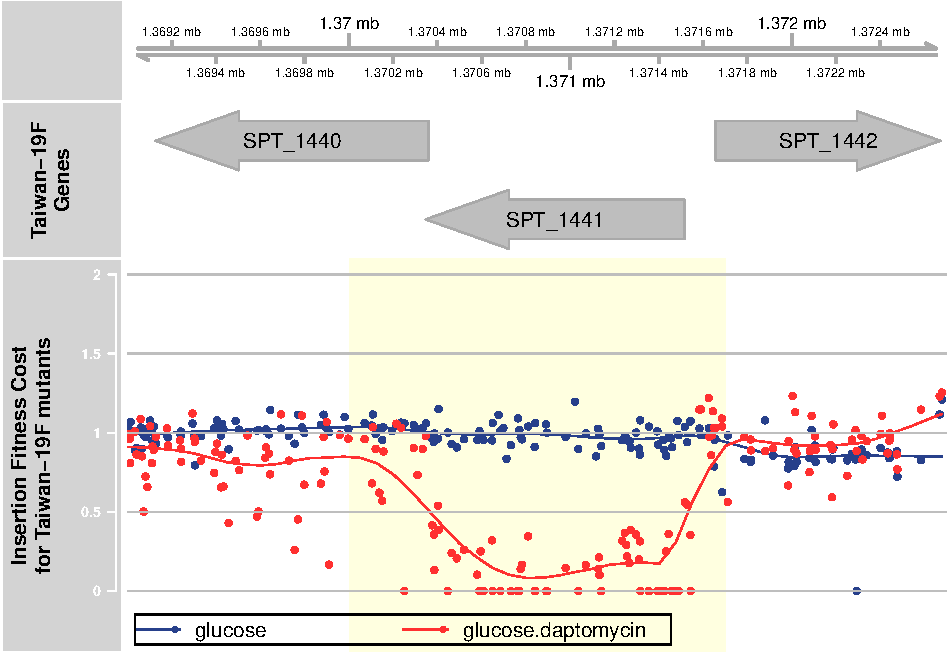
\includegraphics{magentaManual_files/figure-latex/unnamed-chunk-8-1.pdf}

\newpage

\subsection{Single Track Visualization of Tn-Seq
Data}\label{single-track-visualization-of-tn-seq-data}

\begin{Shaded}
\begin{Highlighting}[]
\NormalTok{mainTitle =}\StringTok{ "Taiwan-19F Mutant Fitness in Glucose & Daptomycin"}

\NormalTok{visSingleFit <-}\StringTok{ }\NormalTok{function(ctrlFile, exptFile, x1, x2, h1, h2) \{}
    \NormalTok{ctrl <-}\StringTok{ }\KeywordTok{read.csv}\NormalTok{(ctrlFile)}
    \NormalTok{expt <-}\StringTok{ }\KeywordTok{read.csv}\NormalTok{(exptFile)}
    \KeywordTok{plot}\NormalTok{(ctrl$pos, ctrl$fitness, }\DataTypeTok{xlab =} \StringTok{"Genomic Coordinate"}\NormalTok{, }
        \DataTypeTok{ylab =} \StringTok{"Insertion Fitness Cost"}\NormalTok{, }\DataTypeTok{main =} \NormalTok{mainTitle, }\DataTypeTok{type =} \StringTok{"h"}\NormalTok{, }
        \DataTypeTok{xlim =} \KeywordTok{c}\NormalTok{(x1, x2), }\DataTypeTok{col =} \StringTok{"darkblue"}\NormalTok{)}
    \KeywordTok{legend}\NormalTok{(}\StringTok{"topright"}\NormalTok{, }\FloatTok{1.35}\NormalTok{, }\KeywordTok{c}\NormalTok{(}\StringTok{"Glucose"}\NormalTok{, }\StringTok{"Glucose + Daptomycin"}\NormalTok{), }
        \DataTypeTok{lty =} \KeywordTok{c}\NormalTok{(}\DecValTok{1}\NormalTok{, }\DecValTok{1}\NormalTok{), }\DataTypeTok{lwd =} \KeywordTok{c}\NormalTok{(}\FloatTok{1.5}\NormalTok{, }\FloatTok{2.5}\NormalTok{), }\DataTypeTok{col =} \KeywordTok{c}\NormalTok{(}\StringTok{"darkblue"}\NormalTok{, }
            \StringTok{"red"}\NormalTok{), }\DataTypeTok{bty =} \StringTok{"n"}\NormalTok{, }\DataTypeTok{cex =} \FloatTok{0.6}\NormalTok{)}
    \KeywordTok{abline}\NormalTok{(}\DataTypeTok{h =} \DecValTok{1}\NormalTok{, }\DataTypeTok{col =} \StringTok{"black"}\NormalTok{)}
    \KeywordTok{lines}\NormalTok{(expt$pos, expt$fitness, }\DataTypeTok{col =} \StringTok{"red"}\NormalTok{, }\DataTypeTok{type =} \StringTok{"h"}\NormalTok{)}
    \KeywordTok{rect}\NormalTok{(h1, }\DecValTok{0}\NormalTok{, h2, }\FloatTok{1.3}\NormalTok{, }\DataTypeTok{col =} \StringTok{"#F4FA5840"}\NormalTok{, }\DataTypeTok{border =} \OtherTok{NA}\NormalTok{)}
\NormalTok{\}}
\KeywordTok{visSingleFit}\NormalTok{(ctrlSingleFitFile, exptSingleFitFile, }\DecValTok{1370000}\NormalTok{, }\DecValTok{1372514}\NormalTok{, }
    \DecValTok{1370347}\NormalTok{, }\DecValTok{1371514}\NormalTok{)}
\end{Highlighting}
\end{Shaded}

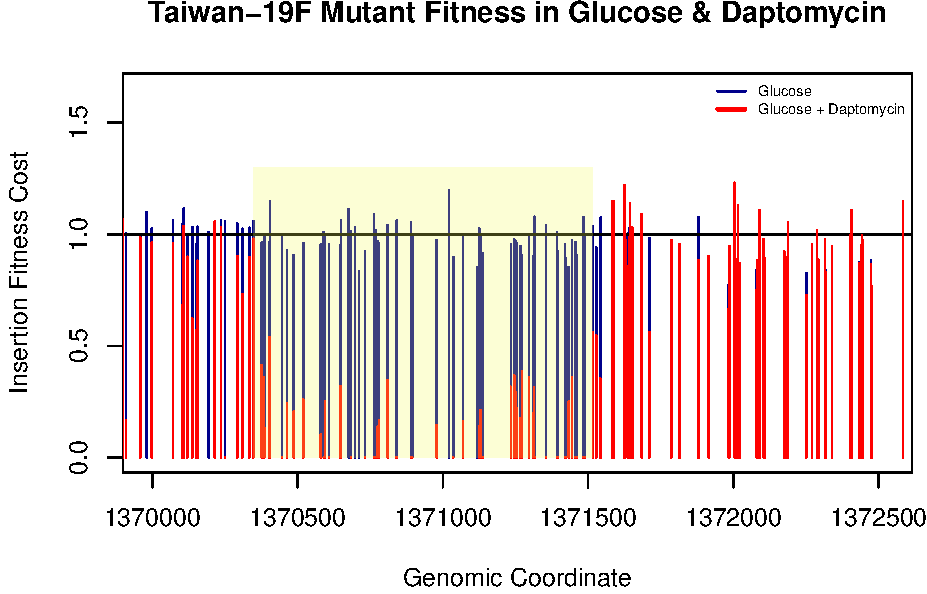
\includegraphics{magentaManual_files/figure-latex/unnamed-chunk-9-1.pdf}

\subsection{Other Examples of Tn-Seq
Data}\label{other-examples-of-tn-seq-data}

\subsubsection{Region with underrepresented number of
insertions}\label{region-with-underrepresented-number-of-insertions}

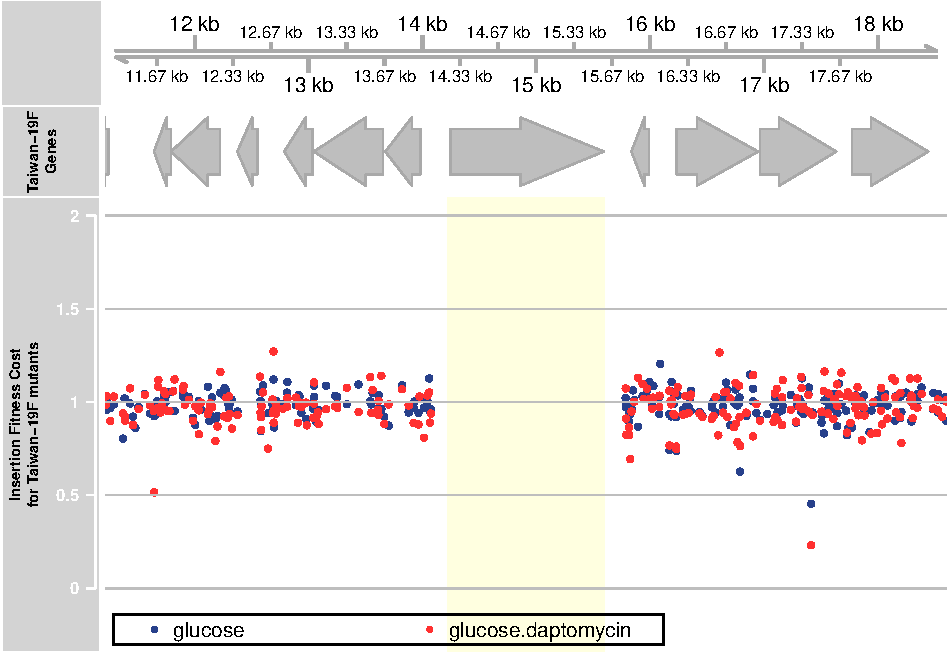
\includegraphics{magentaManual_files/figure-latex/unnamed-chunk-10-1.pdf}


\end{document}
